\documentclass[../main.tex]{subfiles}
\begin{document}
\setchapterstyle{kao}
\setchapterpreamble[u]{\margintoc}
\setchapterimage[6.5cm]{Images/GT.jpg}
\chapter[Gauge Field Theories]{Gauge Field Theories\footnotemark[0]}
\labch{GT}
\section{Particles in the Poincaré Group}
One important symmetry of our universe is that no place in space-time seems to be different from any other place. Therefore, our theory should be \textbf{translation invariant}. Another important symmetry is \textbf{Lorentz invariance}. The group of translations and Lorentz transformations is called the \textbf{Poincaré group} ISO(1,3).\\
We move our attention to particles, which have mass, spin and other quantum numbers. They also have momentum and the projection of spin on some axis. If we rotate or boost to change frame, only the momenta and the spin projection change, but other quantum numbers do not. Hence, a particle can be defined as a set of states that mix only among themselves under Poincaré transformations, denoted by $\pazocal{P}$.
\[
\ket{\Psi}\to\pazocal{P}\ket{\Psi}
\]
A set of objects $\Psi$ that mix under a transformation group is called a \textbf{representation} of the group. If no subset of states transform among themselves then the representation is \textbf{irreducible}. Moreover, we want \textbf{unitary} representations. This is because in field theory we compute matrix elements $\pazocal{M}=\bra{\Psi_1}\ket{\Psi_2}$ which should be Poincaré invariant. If $\pazocal{M}$ is Poincaré invariant and $\ket{\Psi_1}$ and $\ket{\Psi_2}$ transform under a Poincaré transformation $\pazocal{P}$ we find:
\[
\pazocal{M}=\bra{\Psi_1}\pazocal{P}^\dagger\pazocal{P}\ket{\Psi_2}
\]
\marginnote{From \cite{schwartz}, Section 8.1.}So $\pazocal{P}^\dagger\pazocal{P}=1$, which is the definition of unitarity. Unitary representations of the Poincaré group are only a small subset of all the possible representations of it. 
\begin{definition}
Particles transform under irreducible unitary representation of the Poincaré group.
\end{definition}
Unfortunately, there are \textit{no finite-dimensional unitary representations} of the Poincaré group. The \textit{unitary irreducible representations} of the Poincaré group were classified by Wigner: they are all infinite dimensional and described by \textbf{fields}.
% In this chapter, we want to discuss gauge invariance. As a starting point, we give some definitions:
% \begin{itemize}
%     \item \underline{Particle}: unitary infinite-dimensional representation of the Poincaré group
%     \item \underline{Field}: non-unitary finite-dimensional representation of the Lorentz group
% \end{itemize}
% Photons have 2 degrees of freedom, while the field $A_\mu$ has 4: one of them is redundant and it is possible to suppress it using gauge invariance. Requesting Lorentz invariance implying having gauge invariance, hence the latter is not a symmetry. We encounter this type of redundancy in quantum mechanics too, where there are the phases of our states. Here it is the same thing, with just more degrees of freedom. Gauge invariance has no physical implication, it is not associated to any conservation law, it is just a technical instrument that allows us to have local fields.\\
% We want to move from particles to local fields and in order to do that we use the \textbf{method of induced representations} (Wigner), which works for non semi-simple groups: we need an invariant and abelian subgroup. The Lorentz group SO(3,1) does not satisfy this constraint, so we use the group of isomorphisms in the \href{https://en.wikipedia.org/wiki/Hermann_Minkowski}{Minkowski} space ISO(3,1): the Poincaré group.
% \[
% [P^\mu,P^\nu]=0 \quad [M^{\mu\nu},P^\rho]=i(\eta^{\mu\rho}P^\nu-\eta^{\nu\rho}P^\mu)
% \]
% The first commutator tells us that the translations form an abelian subgroup, the second one is invariant, i.e. $U(\Lambda)P^\mu U^{-1}(\Lambda)=\eta^\mu_\nu P^\nu$ with $U(\Lambda)=e^{i\omega_{\mu\nu}M^{\mu\nu}}$. How can the Poincaré group be characterized? There are two Casimir operators:
% \[
% \left\{
% \begin{aligned}
% &P^\mu P_\mu=P^2\xleftarrow[]{}\text{invariant mass}\\
% &W^\mu W_\mu=W^2\xleftarrow[]{}\text{\href{https://en.wikipedia.org/wiki/Pauli-Lubanski_pseudovector}{Pauli-Lubanski} vector}\;W^\mu=\frac{1}{2}\epsilon^{\mu\nu\rho\sigma}M_{\nu\rho}P_\sigma
% \end{aligned}
% \right.
% \]
% Focus now on the invariant mass: the fact that it commutes with all the generators of the algebra implies that if an element of the representation has a certain $P^2$, it will be the same for all the other elements of the same representation. 
\marginnote{From \cite{WKT}, Section 10.4.}The unitary irreducible representation of the Poincaré group can be derived by using the \textbf{method of induced representation}. This method is based on the use of the abelian invariant subgroup of translations T$_4$. The square of the four-momentum is a \textbf{Casimir operator} which commutes with all generators, hence with all group transformations. We define it as:
\[
C_1:=P_\mu P^\mu=P^2=p_0^2-p^2
\]
$C_1$ has the desired properties because it is Lorentz invariant (as the scalar product of $P^\mu$ with itself) and it is also invariant under translations due to the abelian nature of T$_4$. However, its eigenvalue $c_1$ is not positive definite and the irreducible representations of the Lorentz group are labelled by $c_1$. The second Casimir of the Poincaré group comes from the \href{https://en.wikipedia.org/wiki/Pauli-Lubanski_pseudovector}{Pauli-Lubanski} vector:
\[
C_2:=W_\mu W^\mu=W^2 \quad W^\mu=\frac{1}{2}\epsilon^{\mu\nu\rho\sigma}M_{\nu\rho}P_\sigma
\]
We can distinguish among 4 cases:
\begin{enumerate}
    \item null vector $p$: $c_1=0$ and $p^0=\Vec{p}=0$ (vacuum)
    \item time-like $p$: $c_1>0$ (massive particle)
    \item light-like $p$: $c_1=0, p^\mu\neq0$ (massless particle)
    \item space-like $p$: $c_1<0$
\end{enumerate}
\section{One-Particle States}\marginnote{From \cite{W1}, Section 2.5.}
We now consider the classification of one-particle states according to their transformation under the Poincaré group. The components of the energy-momentum four-vector all commute with each other, therefore it is natural to express physical state-vectors in terms of eigenvectors $p^\mu$ of the four-momentum $P^\mu$. We introduce a label $\sigma$ to account for the other degrees of freedom, hence we consider state-vectors with:\marginnote{The label $\sigma$ is purely discrete, since we are working with one-particle states.}
\[
P^\mu\ket{\vec{p},\sigma}=p^\mu\ket{\vec{p},\sigma}
\]
Applying translations to these states results in:
\[
U(1,a)\ket{\vec{p},\sigma}=\exp{-iP^\mu a_\mu}\ket{\vec{p},\sigma}=\exp{-i\Vec{p}\cdot \vec{a}}\ket{\vec{p},\sigma}
\]
We now have to consider how these states transform under Lorentz. The effect of operating with a Lorentz transformation $U(\Lambda,0):=U(\Lambda)$ on $\ket{\vec{p},\sigma}$ is to produce an eigenvector of the four-momentum with eigenvalue $\Lambda p$.
\begin{align*}
P^\mu U(\Lambda)\ket{\vec{p},\sigma}&=U(\Lambda)[U^{-1}(\Lambda)P^\mu U(\Lambda)]\ket{\vec{p},\sigma}=U(\Lambda)(\Lambda^{-1,\mu}_\rho P^\rho)\ket{\vec{p},\sigma}\\
&=\Lambda^\mu_\rho p^\rho U(\Lambda)\ket{\vec{p},\sigma}
\end{align*}
Therefore, $U(\Lambda)\ket{\vec{p},\sigma}$ must be a linear combination of the states $\ket{\Lambda p,\sigma'}$.
\begin{equation}
\labeq{csigma}
U(\Lambda)\ket{\vec{p},\sigma}=\sum_{\sigma'}=C_{\sigma',\sigma}(\Lambda,p)\ket{\Lambda p,\sigma'}
\end{equation}
In general, it is possible by using suitable linear combinations of $\ket{\vec{p},\sigma}$ to choose the labels $\sigma$ in such a way that the matrix $C_{\sigma',\sigma}(\Lambda,p)$ is block diagonal, i.e. so that the states $\ket{\vec{p},\sigma}$ gives a representation of the Poincaré group. Our task now is to work out the structure of the coefficients $C_{\sigma',\sigma}(\Lambda,p)$ in irreducible representations of the Poincaré group. For this purpose, note that the only functions of $p^\mu$ that are left invariant by proper orthochronous Lorentz transformations $\Lambda^\mu_\nu$ are the invariant square $p^2=\eta_{\mu\nu}p^\mu p^\nu$ and the sign of $p^0$ (for $p^2\le0$). For each value of $p^2$ we can choose a standard four-momentum $k^\mu$ and express any $p^\mu$ of this class as:
\[
p^\mu=L^\mu_\nu(p) k^\nu
\]
where $L^\mu_\nu(p)$ is a standard Lorentz transformation which depends on $p^\mu$ and also implicitly on the choice of $k^\mu$. A general state with momentum $\Vec{p}$ is defined as:\marginnote{Up to an arbitrary normalization factor.}
\[
\ket{\Vec{p},\sigma}:=U(L(p))\ket{\Vec{k},\sigma}
\]
So far, we said nothing about how the $\sigma$ labels are related to different momenta. Now we operate with $U(\Lambda)$ on the state previously defined:
\[
U(\Lambda)\ket{\Vec{p},\sigma}=U(\Lambda L(p))\ket{\Vec{k},\sigma}=U(L(\Lambda p))U(L^{-1}(\Lambda p)\Lambda L(p))\ket{\Vec{k},\sigma}
\]
The Lorentz transformation $L^{-1}(\Lambda p)\Lambda L(p)$ takes $k$ to $L(p)k=p$ then to $\Lambda p$ and then back to $k$: it belongs to the subgroup of the Lorentz group consisting of transformations $W^\mu_\nu$ which leave $k^\mu$ invariant. This subgroup is called the \textbf{little group}.\\
We can explicitly show that $\ket{\Vec{p},\sigma}$ are eigenvalues of the momentum.
\begin{align*}
P^\mu\ket{\Vec{p},\sigma}&=P^\mu U(L(p))\ket{\Vec{k},\sigma}=U(L(p))[U^{-1}(L(p))P^\mu U(L(p))]\ket{\vec{k},\sigma}\\
&=U(L(p))L(p)^\mu_\nu p^\nu\ket{\vec{k},\sigma}=U(L(p))L(p)^\mu_\nu k^\nu\ket{\vec{k},\sigma}\\
&=U(L(p))p^\mu\ket{\vec{k},\sigma}=p^\mu\ket{\vec{p},\sigma} \quad \checkmark
\end{align*}
Moreover, we can show that this state is also an eigenstate of the Lorentz transformations:
\begin{align*}
U(\Lambda)\ket{\vec{p},\sigma}&=U(\Lambda)U(L(p))\ket{\vec{k},\sigma}=U(L(\Lambda p))[U^{-1}(L(\Lambda p))U(\Lambda)U(L(p))]\ket{\vec{k},\sigma}\\
&=U(L(\Lambda p))U(W(\Lambda,p))\ket{\vec{k},\sigma}\marginnote{The product of unitary transformations is the unitary transformation of the product, $W(\Lambda,p):=L(\Lambda p)^{-1}\Lambda L(p)$.}
\end{align*}
We look more in details at this transformation $W(\Lambda,p)$.
\begin{align*}
W(\Lambda,p)^\mu_\nu k^\nu&=(L(\Lambda p)^{-1}\Lambda L(p))^\mu_\nu k^\nu=(L(\Lambda p)^{-1}\Lambda)L(p)^\mu_\nu k^\nu=(L(\Lambda p)^{-1}\Lambda)^\mu_\nu p^\nu\\
&=(L(\Lambda p)^{-1})^\mu_\nu(\Lambda p)^\nu=k^\nu
\end{align*}
$W(\Lambda,p)$ leaves $k^\mu$ invariant so it is an element of the little group. For any $W$ in the little group we have:
\begin{equation}
\labeq{Wlg}
U(W(\Lambda,p))\ket{\vec{k},\sigma}=\sum_{\sigma'}D_{\sigma\sigma'}(W(\Lambda,p))\ket{\vec{k},\sigma'}
\end{equation}
We can substitute this result in the equation above.
\[
U(\Lambda)\ket{\vec{p},\sigma}=U(L(\Lambda p))\sum_{\sigma'}D_{\sigma\sigma'}(W(\Lambda,p))\ket{\vec{k},\sigma'}=\sum_{\sigma'}D_{\sigma\sigma'}(W(\Lambda,p))\ket{\vec{p}_\Lambda,\sigma'}
\]
where $(\vec{p}_\Lambda)=(\Lambda p)^i$.\\
The problem of finding the coefficients in \refeq{csigma} has been reduced to the problem of finding the representations of the little group. This approach is called the \textbf{method of induced representations}.
By the usual orthonormalization procedure, we can prove that $D_{\sigma\sigma'}$ is unitary:
\begin{align*}
\bra{\vec{p}',\sigma'}\ket{\vec{p},\sigma}&=(2\pi)^32E_p\delta^3(\vec{p}-\vec{p}')\delta_{\sigma\sigma'}=\bra{\vec{p}',\sigma'}U^{-1}(\Lambda)U(\Lambda)\ket{\vec{p},\sigma}\\
&=\sum_{\hat{\sigma}',\hat{\sigma}}D_{\sigma\hat{\sigma}}D_{\sigma'\hat{\sigma}'}^*\bra{\vec{p}_{\Lambda'},\hat{\sigma}'}\ket{\vec{p}_\Lambda,\hat{\sigma}}=\sum_{\hat{\sigma}',\hat{\sigma}}D_{\sigma\hat{\sigma}}D_{\sigma'\hat{\sigma}'}^*(2\pi)^32E_{p_{\Lambda}}\delta^3(\vec{p}_\Lambda-\vec{p}'_{\Lambda'})\delta_{\hat{\sigma}\hat{\sigma}'}\\
&=\sum_{\hat{\sigma}',\hat{\sigma}}D_{\sigma\hat{\sigma}}D_{\sigma'\hat{\sigma}'}^*(2\pi)^32E_p\delta^3(\vec{p}-\vec{p}')\delta_{\hat{\sigma}\hat{\sigma}'}
\end{align*}
It follows that:
\[
\delta_{\sigma\sigma'}=\sum_{\hat{\sigma}',\hat{\sigma}}D_{\sigma\hat{\sigma}}D_{\sigma'\hat{\sigma}'}^*\delta_{\hat{\sigma}\hat{\sigma}'}=\sum_{\hat{\sigma}}D_{\sigma\hat{\sigma}}D_{\sigma'\hat{\sigma}^*}\Rightarrow\text{$D$ is unitary}
\]
\subsection{Massive States}
For massive states, we make a clever choice and work in the reference system where the massive particle is at rest, i.e. $K^\mu=(m,0,0,0)$. The little group is SO(3), since rotations are the only proper orthochronous Lorentz transformations that leaves at rest a particle with zero momentum. 
% For SO(2) we have just one Casimir, $J^2$, which is the element that commutes with all the other elements in the algebra, $[J^2,J^i]=\exp{iJ^iM^i\theta}=0$. The action of the operator does not change the Casimir:
% \[
% J^2U(R(\theta))\ket{s,\sigma}\underset{\mathclap{\tikz \node {$\uparrow$} node [below=1ex] {\footnotesize they commute };}}{=}U(R(\theta))J^2\ket{s,\sigma}=\hbar^2s(s+1)U(R(\theta))\ket{s,\sigma}
% \]
% $\ket{\Vec{k},\sigma}$ gives us a unitary infinite-dimensional representation of the Poincaré group, the idea is to extend this structure to other states of the representation. 
As seen before, elements of the little group are given by $W(\Lambda,p)=L^{-1}(\Lambda p)\Lambda L(p)$. To calculate this rotation, we have to choose a standard boost $L(p)$ which takes the four-momentum from $K^\mu$ to $P^\mu$. Conveniently, this is chosen as:
\[
\left\{
\begin{aligned}
&L_k^i(p)=\delta_{ik}+(\gamma-1)\hat{p}_i\hat{p}_k\\
&L^i_0(p)=L^0_i(p)=\hat{p}_i\sqrt{\gamma^2-1}\\
&L^0_0(p)=\gamma
\end{aligned}
\right.
\quad \text{where}\;
\left\{
\begin{aligned}
&\hat{p}_i=\frac{p_i}{|\Vec{p}|}\\
&\gamma=\frac{\sqrt{p^2+m^2}}{m}
\end{aligned}
\right.
\]
When $\Lambda^\mu_\nu$ is an arbitrary three-dimensional rotation $\pazocal{R}$, the Wigner rotation $W(\Lambda,p)$ is the same as $\pazocal{R}$ for all $p$. In order to see this, note that the boost $L(p)$ may be expressed as:
\[
L(p)=R(\hat{p})B(|\Vec{p}|)R^{-1}(\hat{p})
\]
where $R(\hat{p})$ is a rotation that takes the three-axis into the direction of $\Vec{p}$, while $B(|\Vec{p}|)$ is defined as:
\[
B(|\Vec{p}|)=\left(\begin{array}{cccc}
    1 & 0 & 0 & 0 \\
    0 & 1 & 0 & 0 \\
    0 & 0 & \gamma & \sqrt{\gamma^2-1} \\
    0 & 0 & \sqrt{\gamma^2-1} & \gamma 
\end{array}\right)
\]
For an arbitrary rotation $\pazocal{R}$ we then have:
\[
W(\pazocal{R},p)=R(\pazocal{R}\hat{p})B^{-1}(|\Vec{p}|){\color{green}R^{-1}(\pazocal{R}\hat{p})\pazocal{R}R(\hat{p})}B(|\Vec{p}|)R^{-1}(\hat{p})
\]
The rotation highlighted in green takes the three-axis into the direction of $\Vec{p}$ then in the direction of $\pazocal{R}\Vec{p}$ and then back to the three-axis, therefore it must be just a rotation by some angle $\theta$ around the three-axis:
\[
R^{-1}(\pazocal{R}\hat{p})\pazocal{R}R(\hat{p})=R(\theta)=\left(\begin{array}{cccc}
    \cos\theta & \sin\theta & 0 & 0 \\
    -\sin\theta & \cos\theta & 0 & 0 \\
    0 & 0 & 1 & 0 \\
    0 & 0 & 0 & 1
\end{array}\right)
\]
$R(\theta)$ commute with $B(|\Vec{p}|)$, which gives us:
\[
W(\pazocal{R},p)=R(\pazocal{R}\hat{p})B^{-1}(|\Vec{p}|)R(\theta)B(|\Vec{p}|)R^{-1}(\hat{p})=R(\pazocal{R}\hat{p})R(\theta)R^{-1}(\hat{p})=\pazocal{R}
\]
Finally, this shows us that states of a moving massive particles have the same transformation under rotations as in non-relativistic quantum mechanics.\\
In order to label our sates, it is possible to use the generators $J^2$ and $J_z$ and, being SO(3) compact, the eigenvalues of these generators are quantized. For these states we only need $K^\mu$, $J^2$ and $J_z$. We can prove that $J^2$ is proportional to the second Casimir $W^\mu=\frac{1}{2}\epsilon^{\mu\nu\rho\sigma}M_{\nu\rho}P_\sigma$. $\sigma$ must be a temporal index while all the other ones are spatial.
\[
W^i=\frac{1}{2}\epsilon^{ijk}M_{jk}\cdot m=J^i\cdot m\xrightarrow[]{}W^2=J^2\cdot m^2
\]
Our state can be labeled as $\ket{\Vec{k},\sigma,m,s}$.\marginnote{In principle, we could have other quantum numbers, like isospin, but they have nothing to do with the Poincaré group.}
\[
\left\{
\begin{aligned}
&P^\mu\ket{\Vec{k},\sigma,m,s}=k^\mu\ket{\Vec{k},\sigma,m,s} \quad \text{where $\Vec{k}=0$ and $k^0=m$}\\
&J^2\ket{\Vec{k},\sigma,m,s}=\hbar^2s(s+1)\ket{\Vec{k},\sigma,m,s}\\
&J_z\ket{\Vec{k},\sigma,m,s}=\hbar\sigma\ket{\Vec{k},\sigma,m,s}
\end{aligned}
\right.
\]
\subsection{Massless States}
We want to repeat the same arguments for one-particle massless states, but in this case it is not so simple because the little group is not trivial like it was before. As we previously did, we start by taking a reference momentum which must be compatible with the light-like nature of the state, so we take $K^\mu=(k,0,0,k)$. We need to find the little group of $K^\mu$: we can perform a boost along the $x$-axis, a rotation in the $xz$ plane and again a boost but in the $z$-axis. We require that this sequence of transformations leaves $K^\mu$ invariant.
\begin{enumerate}
    \item Boost along the $x$-axis:
    \[
    \left(\begin{array}{cccc}
    \gamma & \beta\gamma & 0 & 0 \\
    \beta\gamma & \gamma & 0 & 0 \\
    0 & 0 & 1 & 0 \\
    0 & 0 & 0 & 1 
    \end{array}\right)
    \left(\begin{array}{c}
    k \\
    0 \\
    0 \\
    k
    \end{array}\right)=
    \left(\begin{array}{c}
    \gamma k \\
    \beta\gamma k \\
    0 \\
    k
    \end{array}\right)
    \]
    We obtain an $y$ component that we do not want, to throw it away we perform a rotation.
    \item Rotation in the $xz$ plane $(\sin\theta=\beta, \cos\theta=1/\gamma)$:
    \[
    \left(\begin{array}{cccc}
    1 & 0 & 0 & 0 \\
    0 & \cos\theta & 0 & -\sin\theta \\
    0 & 0 & 1 & 0 \\
    0 & \sin\theta & 0 & \cos\theta 
    \end{array}\right)
    \left(\begin{array}{c}
    \gamma k \\
    \beta\gamma k \\
    0 \\
    k
    \end{array}\right)=
    \left(\begin{array}{c}
    \gamma k \\
    0 \\
    0 \\
    \gamma k
    \end{array}\right)
    \]
    We have an undesired factor $\gamma$, so we make another boost to eliminate it.
    \item Boost along the $z$-axis $(\Tilde{\gamma}=(\gamma^2+1)/2\gamma)$:
    \[
    \left(\begin{array}{cccc}
    \Tilde{\gamma} & 0 & 0 & \Tilde{\beta}\Tilde{\gamma} \\
    0 & 1 & 0 & 0 \\
    0 & 0 & 1 & 0 \\
    \Tilde{\beta}\Tilde{\gamma} & 0 & 0 & \Tilde{\gamma} 
    \end{array}\right)
    \left(\begin{array}{c}
    \gamma k \\
    0 \\
    0 \\
    \gamma k
    \end{array}\right)=
    \left(\begin{array}{c}
    k \\
    0 \\
    0 \\
    k
    \end{array}\right)
    \]
\end{enumerate}
This sequence of transformations leaves the momentum invariant, we can perform the boost along the $x$-axis and then the boost along the $z$-axis or vice-versa. Now we want to find the generators of these transformations which commute with $P$ and that allows us to find the quantum numbers needed to label our states. What we have to do is taking the product of these transformations and make it infinitesimal, assuming that $\beta$ is small. For $\beta\ll1$ we have:
\[
\gamma\simeq1+\frac{1}{2}\beta^2 \quad \sin\theta=\beta \quad \cos\theta=1+\pazocal{O}(\beta^2) \quad \Tilde{\beta}=-\frac{1}{2}\beta^2 \quad \Tilde{\gamma}=1+\pazocal{O}(\beta^2)
\]
To the first order in $\beta$, only the first two transformations make a relevant contribution.\marginnote{For $\beta\ll1$, the matrix of the third transformation becomes the identity at first order in $\beta$.}
\[
\begin{aligned}
&\bullet\text{Boost along the $x$-axis:}&&\left(\begin{array}{cccc}
\gamma & \beta\gamma & 0 & 0 \\
    \beta\gamma & \gamma & 0 & 0 \\
    0 & 0 & 1 & 0 \\
    0 & 0 & 0 & 1 
    \end{array}\right)\underset{\beta\ll1}{\simeq}\left(\begin{array}{cccc}
    1 & \beta & 0 & 0 \\
    \beta & 1 & 0 & 0 \\
    0 & 0 & 1 & 0 \\
    0 & 0 & 0 & 1 
    \end{array}\right)\\
&\bullet\text{Rotation in the $xz$ plane:}&&\left(\begin{array}{cccc}
    1 & 0 & 0 & 0 \\
    0 & \cos\theta & 0 & -\sin\theta \\
    0 & 0 & 1 & 0 \\
    0 & \sin\theta & 0 & \cos\theta 
    \end{array}\right)\underset{\beta\ll1}{\simeq}\left(\begin{array}{cccc}
    1 & 0 & 0 & 0 \\
    0 & 1 & 0 & -\beta \\
    0 & 0 & 1 & 0 \\
    0 & \beta & 0 & 1
    \end{array}\right)
\end{aligned}
\]
When taking the product of the two, what we get is:
\begin{align*}
\Lambda^\mu_\nu&=\left(\begin{array}{cccc}
    1 & \beta & 0 & 0 \\
    \beta & 1 & 0 & 0 \\
    0 & 0 & 1 & 0 \\
    0 & 0 & 0 & 1 
    \end{array}\right)\left(\begin{array}{cccc}
    1 & 0 & 0 & 0 \\
    0 & 1 & 0 & -\beta \\
    0 & 0 & 1 & 0 \\
    0 & \beta & 0 & 1
    \end{array}\right)=\left(\begin{array}{cccc}
    1 & \beta & 0 & 0 \\
    \beta & 1 & 0 & -\beta \\
    0 & 0 & 1 & 0 \\
    0 & \beta & 0 & 1
    \end{array}\right)+\pazocal{O}(\beta^2)\\
    &=\delta^\mu_\nu+i\beta A^\mu_\nu+\pazocal{O}(\beta^2)
\end{align*}
The matrix $A^\mu_\nu$ is defined as:
\[
A^\mu_\nu=\left(\begin{array}{cccc}
    0 & -i & 0 & 0 \\
    -i & 0 & 0 & i \\
    0 & 0 & 0 & 0 \\
    0 & -i & 0 & 0
\end{array}\right)=(K_1+J_2)^\mu_\nu
\]
where we denoted with $K_1$ the generator of the boosts along the $x$-axis and with $J_2$ the generator of the rotations around $\hat{y}$.\\
What other transformations can we do? We can perform a SO(2) rotation in the $xy$ plane or a transformation like the previous one but with the boost along the $y$-axis, defining in this way $B^\mu_\nu$.
\[
B^\mu_\nu=\left(\begin{array}{cccc}
    0 & 0 & -i & 0 \\
    0 & 0 & 0 & 0 \\
    -i & 0 & 0 & i \\
    0 & 0 & -i & 0
\end{array}\right)=(K_2-J_1)^\mu_\nu
\]
In this case, $K_2$ is the generator of the boosts along the $y$-axis and $J_1$ the generator of the rotations around $\hat{x}$.\\
The little group will be composed by three generators, $A^\mu_\nu$, $B^\mu_\nu$ and $J_3$ so in general we have:\marginnote{\[
J_3=\left(\begin{array}{cccc}
    0 & 0 & 0 & 0 \\
    0 & 0 & -i & 0 \\
    0 & +i & 0 & 0 \\
    0 & 0 & 0 & 0
\end{array}\right)
\]}
\[
\Lambda^\mu_\nu=\delta^\mu_\nu+i\alpha A^\mu_\nu+i\beta B^\mu_\nu+i\theta J_3
\]
We found the generators but to identify the group we need to define the algebra. Take these three matrices and compute the commutators, the results we obtain are:
\[
[J_3,A]=iB \quad [J_3,B]=-iA \quad [A,B]=0
\]
$A$ and $B$ commute and they transform one into another under the action of $J_3$: this is an invariant subgroup. There will surely be SO(2) generated by $J_3$ plus another invariant subgroup generated by $A$ and $B$. If we put them in a vector, we observe that it is a translation, so we have rotation+translation. This is the \textbf{group of isomorpshims} in $\mathbb{R}^2$ called ISO(2) which is not compact\marginnote{The Poincaré group is the group of isomorphism in Minkowski space, denoted by ISO(3,1).}.\\
We have to find the unitary representation of this group but, as in the Poincaré case, being it not compact we have the problem that this unitary representation will not be finite-dimensional. However, we have an invariant subgroup, so it is possible to use the method of induced representations but we need to find the Casimir first. So far, we have just one Casimir $P^2=A^2+B^2$ with $\vec{P}=(A,B)$. As in the massless case, this corresponds to the second Casimir of the Poincaré group, which is the square of the Pauli-Lubanski vector $W^\mu$: now we restrict it to states with $P^\mu=K^\mu=(k,0,0,k)$.
\[
\left\{
\begin{aligned}
&W^0=\frac{1}{2}(\epsilon^{0123}M_{12}k+\epsilon^{0213}M_{21}k)=M_{12}\cdot k=J_3\cdot k\marginnote{$J_i=M_{kl}$, with $i,k,l$ symmetric permutations of 123.}\\
&W^1=\frac{1}{2}(\epsilon^{1230}M_{23}k+\epsilon^{1320}M_{32}k+\epsilon^{1203}M_{20}k+\epsilon^{1023}M_{02}k)=k(-J_1+K_2)=+k\cdot B\\
&W^2=\frac{1}{2}(\epsilon^{2130}M_{13}k+\epsilon^{2310}M_{31}k+\epsilon^{2013}M_{01}k+\epsilon^{2103}M_{10}k)=k(-J_2-K_1)=-k\cdot A\\
&W^3=\frac{1}{2}(\epsilon^{3210}M_{21}k+\epsilon^{3120}M_{12}k)=-k\cdot J_3
\end{aligned}
\right.
\]
We take the square, $W_\mu W^\mu=W^2=-k^2(A^2+B^2)$. We want to classify physical states according to the value of the Casimir, there are two types of states, which can be classified as $\ket{\Vec{P}}=\ket{a,b}$, where $a$ and $b$ are eigenvalues of $A$ and $B$.
\begin{enumerate}
    \item $|\vec{P}|^2=A^2-B^2>0$: $\ket{a,b}$ are real numbers giving an infinite number of states. These states are not observed in nature, because there are no massless particles with continuous indices, they are all described by discrete quantities. Hence, this case is only possible from a mathematical point of view.
    \item $|\vec{P}|^2=A^2+B^2=0$: $\ket{a,b}=\ket{0,0}$, it is not possible to apply translations and we can only do rotations since they leave this vector invariant. The little group of (0,0) is SO(2). These states are distinguished by the eigenvalue $\sigma$ of the remaining generator $J_3$. Since the momentum $\Vec{k}$ is in the third direction, $\sigma$ gives the component of angular momentum in the direction of motion, called \textbf{helicity}
\end{enumerate}
We are now able to calculate the Lorentz transformation properties of general massless particle states. We know what is an arbitrary element  $W$ of the little group, so we can write:
\[
U(W)\ket{\vec{k},\sigma}=\exp{i\alpha A+i\beta B+i\theta J_3}\ket{k,\sigma}=\exp{i\theta\sigma}\ket{\vec{k},\sigma}
\]
Therefore, \refeq{Wlg} tells us that:
\[
D_{\sigma'\sigma}(W)=\exp{i\theta\sigma}\delta_{\sigma'\sigma}
\]
What are the possible values of the helicity $h$? We have just seen that the action of the little group on physical states is just a rotation around the momentum and there is no \textit{algebraic} reason for a limitation to integer or half-integer values. However, there is a \textit{topological} reason: a rotation by an angle 4$\pi$ around the momentum cannot be continuously deformed into any rotation, so the factor $\exp{4\pi i\sigma}$ must be unity, hence $\sigma$ has to be either integer or half-integer. Note that helicity is Lorentz invariant: a massless particle of a given $\sigma$ looks the same in all inertial frames (aside from its momentum). We would be justified in thinking of massless particles of different helicity as different species of particles. States with $h=1$ belong to a different representation from states with $h=-1$, they are basically different particles. Why don't we use different names? Because, for example, electromagnetic interaction is invariant under parity, which flips the sign of the helicity: for a photon with helicity +1 there will be a photon with helicity -1. The same reasoning applies for gravitational interaction, with the supposed \textit{gravitino} with helicity $\pm2$. On the other hand, massless particles of helicity $\pm\frac{1}{2}$ emitted in nuclear beta decay have no interactions that respect parity, so they are given different names: neutrinos for helicity $+\frac{1}{2}$ and anti-neutrinos for helicity $-\frac{1}{2}$.\\
% We have the combination CPT and we want to see how helicity transforms under it:
% \begin{table}[h]
%     \centering
%     \begin{tabular}{c|ccc}
%      & Spin$(\vec{s})$ & Momentum $(\vec{p})$ & Helicity $(\vec{s}\cdot\vec{p}/|\vec{p}|)$ \\
%      \hline
%      P & +1 & -1 & -1 \\
%      C & +1 & +1 & +1 \\
%      T & -1 & -1 & +1 \\
%      CPT & -1 & +1 & -1 \\
%      \hline
%     \end{tabular}
%     \caption*{}
%     \label{tab:my_label}
% \end{table}\\
% \noindent
% We see that helicity changes sign under P, so it changes sign under CPT too. If we have a particle with a certain charge and helicity, there must exist another particle with opposite charge and opposite helicity. Are there other massless particles in nature? For a while, it was believed that the neutrino was massless but now we know that they have a small mass. Neutrino and anti-neutrino have different names because they interact via weak interaction which does not conserve parity. We want to understand what type of neutrinos we have in nature.
% \begin{itemize}
%     \item \underline{Massive neutrinos}: they have 2 degrees of freedom (given by the $z$ component of the spin) and no charge, neutrinos and anti-neutrinos are equal because there is no charge to distinguish them. In terms of fields, they are described by real Majorana fields, hence only one creation/annihilation operator. Another possibility is to have them charged with 4 degrees of freedom: the $z$ component of the spin and the opposite charge between neutrinos and anti-neutrinos. In this case, we need Dirac creation and annihilation operators.
%     \item \underline{Massless neutrinos (old version)}: they are charged with 2 degrees of freedom, having them being charged is the reason why it was impossible to have the Majorana mass term. We know, due to oscillations, that they must have a mass, but we don't know yet whether is the Majorana one or the Dirac one.
% \end{itemize}
% We want to generate states with arbitrary momentum and we do that using Lorentz transformations: $\ket{\vec{p},h}:=U(L(p))\ket{\vec{k},h}$, with $U(L(p))$ being a boost+rotation. If we are in a reference system such that $K^\mu=(k,0,0,k)$, this means that the boost is along the $z$-axis and then we make the rotation.
In the massive case, the matrix $D_{\sigma\sigma'}$ mixes the spin indices, so $\sigma$ is not invariant under Lorentz transformations, there is a multiplet of components which mix under Lorentz. In the massless case, helicity does not mix and it is really Lorentz invariant.
% \subsection{Vacuum in the Poincaré Group}
% We want to justify the fact that the vacuum is described by $P^2=0$ and $P^\mu=0$: what kind of states can we have with zero momentum? We have to use the induced representations method and see what is the little group which leaves $P^\mu=0$ invariant. This is SO(3,1): what are the unitary representations of SO(3,1)? We have two possibilities:
% \begin{center}
% \begin{tikzcd}
% &\text{singlet representations (unitary and 1-dimensional)=vacuum}\\
% \text{SO}(3,1)\arrow[ru] \arrow[rd] \\
% &\text{non trivial $\infty$-dimensional representations=not realized in nature}
% \end{tikzcd}
% \end{center}
% The vacuum is the only possible state such that $P^\mu\ket{0}=0$, it is a singlet in the Poincaré group with zero energy.
\section{Lorentz Covariant Local Fields}\marginnote{From \cite{W1}, Section 5.1 and Section 5.3.}
Starting from representations derived in the previous section, our idea is to construct fields which are solutions of the equations of motion in the non-interactive case.\marginnote{I assume the choice of working in the non-interactive case is just for simplicity.} We then start from particles to construct fields which properly transforms under Lorentz. Our main attention is vectorial fields, but it is the same for other fields too. We already know that fields are written in terms of creation and annihilation operators, so we want to find transformation rules for these operators which will automatically apply for the fields.\\
\subsection{Massive Case}
Consider now the massive case\marginnote{Same arguments apply for the massless case.}, we saw that states transform as:
\[
U(\Lambda)\ket{\vec{p},\sigma}=\sum_{\sigma'}D_{\sigma\sigma'}W(\Lambda,p)\ket{\vec{p}_\Lambda,\sigma'}
\]
We define the creation operator and its commutation rules:
\[
a^\dagger(\vec{p},\sigma)\ket{0}=\frac{1}{\sqrt{2E_p}}\ket{\vec{p},\sigma} \quad [a(\vec{p}',\sigma'),a^\dagger(\vec{p},\sigma)]=(2\pi)^3\delta^3(\vec{p}-\vec{p}')\delta_{\sigma\sigma'}
\]
The next step is to write the transformation rule for the states but using the creation operator:
\begin{align*}
U(\Lambda)\ket{\vec{p},\sigma}&=\sqrt{2E_p}U(\Lambda)a^\dagger(\vec{p},\sigma)\ket{0}=\sqrt{2E_p}[U(\Lambda)a^\dagger(\vec{p},\sigma)U^{-1}(\Lambda)]\ket{0}\marginnote{The vacuum is invariant under Lorentz.}\\
&=\sum_{\sigma'}D_{\sigma\sigma'}\sqrt{2E_{p_\Lambda}}a^\dagger(\vec{p}_\Lambda,\sigma')\ket{0}
\end{align*}
Comparing the two lines in the expression above, we find:
\[
\left\{
\begin{aligned}
&U(\Lambda)a^\dagger(\vec{p},\sigma)U^{-1}(\Lambda)=\sqrt{\frac{E_{p_\Lambda}}{E_p}}\sum_{\sigma'}D_{\sigma\sigma'}a^\dagger(\vec{p}_\Lambda,\sigma')\\
&U(\Lambda)a(\vec{p},\sigma)U^{-1}(\Lambda)=\sqrt{\frac{E_{p_\Lambda}}{E_p}}\sum_{\sigma'}D_{\sigma\sigma'}^*a(\vec{p}_\Lambda,\sigma')
\end{aligned}
\right.
\]
% Repeating more or less the same arguments, for massless particles one obtains:
% \[
% \left\{
% \begin{aligned}
% &U(\Lambda)a^\dagger(\vec{p},h)U^{-1}(\Lambda)=\sqrt{\frac{E_{p_\Lambda}}{E_p}}\exp{-ih\theta(\Lambda,\vec{p})}a^\dagger(\vec{p}_\Lambda,h)\\
% &U(\Lambda)a(\vec{p},h)U^{-1}(\Lambda)=\sqrt{\frac{E_{p_\Lambda}}{E_p}}\exp{-ih\theta(\Lambda,\vec{p})}a(\vec{p}_\Lambda,h)
% \end{aligned}
% \right.
% \]
Take now a massive vectorial field:
\[
V^\mu(x)=\sum_{\sigma=0,\pm1}\int\frac{d^3p}{(2\pi)^3}\frac{1}{\sqrt{2E_p}}\left[a(\vec{p},\sigma)\varepsilon^\mu(\vec{p},\sigma)e^{-ipx}+a^\dagger(\vec{p},\sigma)\varepsilon^{\mu*}(\vec{p},\sigma)e^{+ipx}\right]
\]
When we transform it, we require that $U(\Lambda)V^\mu(x)U^{-1}(\Lambda)=(\Lambda^{-1})^\mu_\nu V^\nu(\Lambda x)$, i.e. it transforms as a Lorentz four-vector. In order to get this result, we need to impose some kind of transformation rules on the polarization vector $\varepsilon^\mu(\vec{p},\sigma)$.
\[
\left\{
\begin{aligned}
&U(\Lambda)V^\mu(x)U^{-1}(\Lambda)=\sum_{\sigma\sigma'}\int\frac{d^3p}{(2\pi)^3}\frac{1}{\sqrt{2E_p}}\sqrt{\frac{E_{p_\Lambda}}{E_p}}\left[D_{\sigma\sigma'}^*\varepsilon^\mu(\vec{p},\sigma)a(\vec{p}_\Lambda,\sigma')e^{-ipx}+\text{h.c.}\right]\\
&(\Lambda^{-1})^\mu_\nu V^\nu(\Lambda x)=\sum_{\sigma'}\int\frac{d^3p_\Lambda}{(2\pi)^3}\frac{1}{\sqrt{2E_{p_\Lambda}}}[(\Lambda^{-1})^\mu_\nu\varepsilon^\nu(\Vec{p}_\Lambda,\sigma')a(\Vec{p}_\Lambda,\sigma')e^{-i(\Lambda p)(\Lambda x)}+\text{h.c.}]
\end{aligned}
\right.
\]
Comparing the two expressions above, we have to impose that:\marginnote{The integral measure is Lorentz invariant, so:
\[
\int\frac{d^3p}{E_p}=\int\frac{d^3p_\Lambda}{E_{p_\Lambda}}
\]}
\[
\sum_\sigma D_{\sigma\sigma'}^*\varepsilon^\mu(\vec{p},\sigma)=(\Lambda^{-1})^\mu_\nu\varepsilon^\nu(\vec{p}_\Lambda,\sigma')
\]
If we look at the condition we imposed over $\varepsilon^\mu(\vec{p},\sigma)$, it is possible to see that there are two indices which transform under Lorentz, $\mu$ and $\sigma$. $\mu$ transforms with $\Lambda$, which is what we expect for a vector, but also $\sigma$ transforms and it has nothing to do with the field. $\sigma$ is the index for particles and it transforms as a representation of the little group: $\varepsilon^\mu(\vec{p},\sigma)$ is the object connecting particles and fields.\\
We would like to find an explicit expression for $\varepsilon^\mu(\vec{p},\sigma)$, to do that we work in the reference frame where the particle is at rest, $\Vec{p}=0$. Let $\Lambda$ be the standard boost $L(q)$ that takes a particle of mass $m$ from rest to some four-momentum $q^\mu$. It follows that $L(p)=\mathbb{1}$ and:
\[
W(\Lambda,p)=L^{-1}(\Lambda p)\Lambda L(p)=L^{-1}(q)L(q)=\mathbb{1}
\]
This implies that $D_{\sigma\sigma'}(W)=D_{\sigma\sigma'}(\mathbb{1})=\delta_{\sigma\sigma'}$, so in this special case we get:
\[
\varepsilon^\mu(0,\sigma)=(L^{-1}(q))^\mu_\nu\varepsilon^\nu(\vec{q},\sigma)\xleftrightarrow[]{}\varepsilon^\mu(\vec{q},\sigma)=L(q)^\mu_\nu\varepsilon^\nu(0,\sigma)
\]
In other words, if we know the expression for the polarization vector in the reference system where the particle is at rest, then know the expression for the polarization vector in any reference system by simply performing a boost.\\
Now, keep working with $\Vec{p}=0$ but this time let $\Lambda$ be a Lorentz transformation with $\Vec{p}_\Lambda=0$, i.e. take $\Lambda$ as a rotation $R$. The rotation acts on the spatial components which are all equal to zero, hence $L(\Lambda k)=L(k)=1$ so $W=\Lambda=R$. We substitute it:
\[
\sum_\sigma D_{\sigma\sigma'}^*(R)\varepsilon^\mu(0,\sigma)=(R^{-1})^\mu_\nu\varepsilon^\nu(0,\sigma')
\]
and we obtain the transformation rule.\marginnote{Note that $D_{\sigma\sigma'}^*=(D^\dagger)_{\sigma\sigma'}=(D^{-1})_{\sigma\sigma'}$.}
\begin{equation}
\labeq{transfrule}
R^\mu_\nu\varepsilon^\nu(0,\sigma)=\sum_{\sigma'}D_{\sigma\sigma'}(R)\varepsilon^\mu(0,\sigma')
\end{equation}
What we want to describe are particles with spin 1 and field $V^\mu(x)$, therefore $D_{\sigma\sigma'}$ is a representation of rotations with spin 1. $R^\mu_\nu$ is a representation of the rotations but it is not irreducible: $\Lambda^\mu_\nu$ is a 4-vector of SO(3,1), i.e. a $3\oplus1$ of SO(3). Why $3\oplus1$?
% \[
% P^\mu=\left(\begin{array}{c}
%     p^0 \\
%     p^1 \\
%     p^2 \\
%     p^3
% \end{array}\right)
% \begin{array}{c}
%     \}1\\
% \end{array}
% \]
\[
P^\mu=\left(\begin{array}{c}
    p^0\\
    p^1\\
    p^2\\
    p^3
    \end{array}\right)
\setstackgap{L}{1.2\normalbaselineskip}
\vcenter{\hbox{\stackunder[-1pt]{
  \left.{\Centerstack{}}\right\}1\to\text{singlet under rotations}
}{
  \left.{\Centerstack{\\ \\}}\right\}3\to\text{triplet under rotations}
}}}
\]
Another way to see it explicitly is to look directly at the generators of this rotation:
\[
(J_1)^\mu_\nu=\left(\begin{array}{c:ccc}
    0 & 0 & 0 & 0 \\
    \hdashline
    0 & 0 & 0 & 0 \\
    0 & 0 & 0 & -i \\
    0 & 0 & +i & 0 \\
\end{array}\right)
\quad 
(J_2)^\mu_\nu=\left(\begin{array}{c:ccc}
    0 & 0 & 0 & 0 \\
    \hdashline
    0 & 0 & 0 & +i \\
    0 & 0 & 0 & 0 \\
    0 & -i & 0 & 0 \\
\end{array}\right)
\quad 
(J_3)^\mu_\nu=\left(\begin{array}{c:ccc}
    0 & 0 & 0 & 0 \\
    \hdashline
    0 & 0 & -i & 0 \\
    0 & +i & 0 & 0 \\
    0 & 0 & 0 & 0 \\
\end{array}\right)
\]
The only non-zero components are the one in the $3\times3$ subgroup. $\varepsilon^\mu$ must transform as spin 1, so as a triplet, therefore it cannot have temporal component since it would be a singlet that we do not want. If we now take an \textbf{infinitesimal} transformation we have:
\[
\left\{
\begin{aligned}
&R^\mu_\nu=\delta^\mu_\nu+i\theta\hat{n}(\vec{J})^\mu_\nu\xleftarrow[]{}\text{$4\times4$ generators}\\
&D_{\sigma\sigma'}(R)=\delta_{\sigma\sigma'}+i\theta\hat{n}(\vec{J})_{\sigma\sigma'}\xleftarrow[]{}\text{$3\times3$ representation}
\end{aligned}
\right.
\]
We put all of this in the transformation rule we found [\refeq{transfrule}] and we get:
\[
(\vec{J})^\mu_\nu\varepsilon^\nu(0,\sigma)=\sum_{\sigma'}(\vec{J})_{\sigma\sigma'}\varepsilon^\mu(0,\sigma')
\]
Now we can be smart and make a clever choice, selecting $\mu=0$ since $J^0_\nu=0$ and obtaining $\varepsilon^0(0,\sigma')=0$.\marginnote{This is because $(\vec{J})_{\sigma\sigma'}\neq0$.} This is the condition for massive particles: we have 3 degrees of freedom and $\varepsilon$ has 4, so one of them must be zero, the singlet. It is now possible to choose a basis:
\[
\varepsilon^\mu(0,0)=\left(\begin{array}{c}
    0 \\
    0 \\
    0 \\
    +1
\end{array}\right)
\quad
\varepsilon^\mu(0,+1)=\frac{1}{\sqrt{2}}\left(\begin{array}{c}
    0 \\
    +1 \\
    +i \\
    0
\end{array}\right)
\quad
\varepsilon^\mu(0,-1)=\frac{1}{\sqrt{2}}\left(\begin{array}{c}
    0 \\
    +1 \\
    -i \\
    0
\end{array}\right)
\]
From this, it is possible to see that:
\[
\left\{
\begin{aligned}
&\varepsilon^\mu(0,\sigma)\varepsilon_\mu(0,\sigma')=-\delta_{\sigma\sigma'}\\
&\varepsilon^\mu(0,\sigma)K_\mu=0
\end{aligned}
\right.
\]
where $K^\mu=(m,0,0,0)$. These conditions hold true also for a generic momentum $P^\mu$, with the last one giving the condition on the fields $\partial_\mu V^\mu(x)=0$. We can show that this comes from the equations of motion. In order to do that, take a Lagrangian for massive spin-1 field:\marginnote{From \cite{schwartz}, Section 8.2.2.}
\[
\pazocal{L}=-\frac{1}{2}(\partial_\nu A_\mu)(\partial_\nu A_\mu)+\frac{1}{2}m^2A_\mu^2
\]
where $A_\mu^2=A_\mu A^\mu$. The equations of motion are $(\Box+m^2)A_\mu=0$ which have four propagating modes. In fact, this is not a Lagrangian for a massive spin-1 field but rather the Lagrangian for four massive scalar fields $A_0, A_1, A_2, A_3$. That is, we have $4=1\oplus1\oplus1\oplus1$ which is not what we wanted. There is one more Lorentz-invariant kinetic term e can write down, which is $A_\mu\partial_\mu\partial_\nu A_\nu$. The most general free Lagrangian is:
\[
\pazocal{L}=\frac{a}{2}A_\mu\Box A_\mu+\frac{b}{2}A_\mu\partial_\mu\partial_\nu A_\nu+\frac{1}{2}m^2A_\mu^2
\]
where $a$ and $b$ are numbers. As long as $b$ is non-zero, the $\partial_\mu A_\mu$ contraction forces $A_\mu$ to transform as a four-vector because if it transformed as four scalars, $\partial_\mu A_\mu$ would not be Lorentz invariant. We should now have $4=3\oplus1$ and have a chance to get rid of the degree of freedom corresponding to spin 0, isolating the three degrees of freedom for a spin-1 particle. The equations of motion are:
\[
a\Box A_\mu+b\partial_\mu\partial_\nu A_\nu+m^2A_\mu=0
\]
Taking $\partial_\mu$ of this equation gives us:
\[
[(a+b)\Box+m^2](\partial_\mu A_\mu)=0
\]
If $a=-b$ and $m\neq0$, this reduces to $\partial_\mu A_\mu=0$, which removes one degree of freedom. Since $\partial_\mu A_\mu=0$ is a Lorentz-invariant condition, it has to remove a complete representation which with one degree of freedom can only be the spin-0 component. Taking $a=1$ and $b=-1$, we find:
\[
\pazocal{L}=-\frac{1}{4}F_{\mu\nu}^2+\frac{1}{2}m^2A_\mu^2
\]
This is called the \href{https://en.wikipedia.org/wiki/Alexandru_Proca}{Proca} Lagrangian. Here we did not say anything about gauge invariance or electromagnetism, we just derived that $F_{\mu\nu}$ appears based on constructing a Lagrangian that generates a constraint to propagate only the spin-1 field by removing the spin-0 field. Equations of motion now imply $(\Box+m^2)A_\mu=0$ and $\partial_\mu A_\mu=0$.
\subsection{Massless Case}\marginnote{From \cite{W1}, Section 5.9.}
We want to repeat the same story for the massless case, so we start by constructing a general free field for a massless particle as a linear combination of creation and annihilation operators. In this case, the transformation rule is:
\[
U(\Lambda)a(\vec{p},h)U^{-1}(\Lambda)=\exp{-ih\theta(\Lambda,p)}a(\vec{p}_\Lambda,h)\sqrt{\frac{E_{p_\Lambda}}{E_p}}
\]
As we previously did, we are looking for the transformation rule of the field, $U(\Lambda)A^\mu(x)U^{-1}(\Lambda)\stackrel{?}{=}(\Lambda^{-1})^\mu_\nu A^\nu(x)$. This is not possible and we are going to see why.
\[
U(\Lambda)A^\mu(x)U^{-1}(\Lambda)=\sum_{h=\pm1}\int\frac{d^3p}{(2\pi)^3}\frac{1}{\sqrt{2E_p}}\sqrt{\frac{E_{p_\Lambda}}{E_p}}\left[e^{-ih\theta(\Lambda,p)}a(\vec{p}_\Lambda,h)\varepsilon^\mu(\vec{p},h)e^{-ipx}+\text{h.c.}\right]
\]
For the polarization vector $\varepsilon^\mu$, the transformation rule we would like to have is:
\[
e^{-ih\theta(\Lambda,p)}\varepsilon^\mu(\vec{p},h)=(\Lambda^{-1})^\mu_\nu\varepsilon^\nu(\vec{p}_\Lambda,h)
\]
If this holds true, we obtain for the field the desired transformation rule and we are of course happy. Is it possible to realize this transformation? Repeat the same steps of the massive case:
\begin{enumerate}
    \item choose $\Vec{p}=0\Rightarrow L(p)=\mathbb{1}$
    \item choose $\Lambda=L(q)$, since $K^\mu=(k,0,0,k)$ we must perform a boost in the $z$ direction and then a rotation:
    \[
    L(q)\cdot k=q\Rightarrow W(L(q),k)=\mathbb{1}\Rightarrow\theta(\Lambda,p)=0
    \]
    If the transformation of the little group is the identity then we have no phase.
    \[
    \varepsilon^\mu(\vec{k},h)=(L^{-1}(q))^\mu_\nu\varepsilon^\nu(\vec{q},h)\xleftrightarrow[]{}\varepsilon^\mu(\vec{q},h)=L(q)^\mu_\nu\varepsilon^\nu(\vec{k},h)
    \]
    \item choose $\Lambda$ to be an element of the little group of $K^\mu$: $W(\Lambda,p)=\Lambda$
\end{enumerate}
At this point, there are two types of transformations one can do: SO(2) rotations or $S(\alpha,\beta)$, i.e. transformations made by exponentiating the generators $A$ and $B$.\\
In the first case $\Lambda=R(\theta)=\exp{i\theta J_3}$, so we have:
\begin{equation}
\labeq{case1}
R(\theta)^\mu_\nu\varepsilon^\nu(\vec{k},h)=e^{ih\theta}\varepsilon^\mu(\vec{k},h)
\end{equation}
For the second case, $S(\alpha,\beta)^\mu_\nu$ is defined as:
\begin{equation}
\labeq{case2}
S(\alpha,\beta)^\mu_\nu=\left(\begin{array}{cccc}
    1+\xi & \alpha & \beta & -\xi \\
    \alpha & 1 & 0 & -\alpha \\
    \beta & 0 & 1 & -\beta \\
    \xi & \alpha & \beta & 1-\xi
\end{array}\right) \quad S(\alpha,\beta)^\mu_\nu\varepsilon^\nu(\vec{k},h)=\varepsilon^\mu(\vec{k},h)
\end{equation}
where $\xi=\frac{1}{2}(\alpha^2+\beta^2)$. We want to understand how to satisfy both requirements, \refeq{case1} and \refeq{case2}. We start by looking at solutions of the first case and see if they are simultaneously solutions for the other case. Here we will have the two transverse polarizations which are eigenstates of the rotation operator:\marginnote{\[
R(\theta)^\mu_\nu=\left(\begin{array}{cccc}
    1 & 0 & 0 & 0 \\
    0 & \cos\theta & -\sin\theta & 0\\
    0 & \sin\theta & \cos\theta & 0 \\
    0 & 0 & 0 & 1
\end{array}\right)
\]}
\[
\varepsilon^\mu(\vec{k},+1)=\frac{1}{\sqrt{2}}\left(\begin{array}{c}
    0 \\
    +1 \\
    +i \\
    0
\end{array}\right)
\quad
\varepsilon^\mu(\vec{k},-1)=\frac{1}{\sqrt{2}}\left(\begin{array}{c}
    0 \\
    +1 \\
    -i \\
    0
\end{array}\right)
\]
Are they solutions of \refeq{case2}? The answer is NO.
\[
\left(\begin{array}{cccc}
    1+\xi & \alpha & \beta & -\xi \\
    \alpha & 1 & 0 & -\alpha \\
    \beta & 0 & 1 & -\beta \\
    \xi & \alpha & \beta & 1-\xi
\end{array}\right)\frac{1}{\sqrt{2}}\left(\begin{array}{c}
    0 \\
    +1 \\
    \pm i \\
    0
\end{array}\right)=\frac{1}{\sqrt{2}}\left(\begin{array}{c}
    \alpha\pm i\beta \\
    +1 \\
    \pm i \\
    \alpha\pm i\beta
\end{array}\right)\left\{
\begin{aligned}
&\neq\varepsilon^\mu(\vec{k},\pm1)\\
&=\varepsilon^\mu(\vec{k},\pm1)+\frac{\alpha\pm i\beta}{\sqrt{2}}\frac{K^\mu}{k}
\end{aligned}
\right.
\]
Nonetheless, it is still possible to choose solutions of \refeq{case1}, because we know they solve equations of motion, but also solutions of \refeq{case2} with the extra-term proportional to the momentum. Take now $\Lambda=S(\alpha,\beta)R(\theta)$, we can write the two transformations as:
\[
\Lambda^\mu_\nu\varepsilon^\nu(\vec{k},\pm1)=e^{\pm i\theta}\left(\varepsilon^\mu(\vec{k},\pm1)+\frac{\alpha\pm i\beta}{\sqrt{2}}\frac{K^\mu}{k}\right)
\]
Suppose this is the transformation rule, we want the expression for a transformation of $\varepsilon$ with a generic momentum.
\begin{align*}
\Lambda^\mu_\nu\varepsilon^\nu(\vec{p},\pm1)&=\left(L(\Lambda p)W(\Lambda,p)L^{-1}(p)\right)^\mu_\nu\varepsilon^\nu(\vec{p},\pm1)=\left(L(\Lambda p)W(\Lambda,p)\right)^\mu_\nu\varepsilon^\nu(\vec{k},\pm1)\\
&=(L(\Lambda p))^\mu_\nu e^{\pm i\theta}\left(\varepsilon^\mu(\vec{k},\pm1)+\frac{\alpha\pm i\beta}{\sqrt{2}}\frac{K^\mu}{k}\right)=e^{\pm i\theta}\varepsilon^\mu(\vec{p}_\Lambda,\pm1)+\frac{\alpha\pm i\beta}{\sqrt{2}}\frac{(\Lambda p)^\mu}{k}
\end{align*}
Now we multiply both sides by $(\Lambda^{-1})^\mu_\nu$ and bring the phase to the LHS.
\[
e^{\mp i\theta}\varepsilon^\mu(\vec{p},\pm1)=(\Lambda^{-1})^\mu_\nu\varepsilon^\nu(\vec{p}_\Lambda,\pm1)+\frac{\alpha\pm i\beta}{\sqrt{2}}\frac{P^\mu}{k}
\]
We repeat the same steps of the massive case to find the transformation rule for the field:
\[
U(\Lambda)A^\mu(x)U^{-1}(\Lambda)=(\Lambda^{-1})^\mu_\nu A^\nu(x)+\partial^\mu\lambda_\Lambda(x)
\]
where $\lambda_\Lambda$ is a linear combination of creation and annihilation operators whose precise form does not concern us for the moment.\\ 
\textit{Gauge invariance appeared as a consequence of our request to have the Lagrangian Lorentz invariant.}\\
We have $K^\mu\varepsilon_\mu(\vec{k},\pm1)=0$, if we move to a generic reference system $P^\mu\varepsilon_\mu(\vec{p},\pm1)=0$. Moreover, $\varepsilon^0(\vec{k},\pm1)=0$ is still valid in any reference system. To transform the polarization vector, we need a boost along the $z$ direction and a rotation. The boost acts only on the temporal and third components, hence $\varepsilon^\mu$ remains unchanged under this transformation. What is modified is $K^\mu$, but the orthogonality condition is still valid after the rotation, because if the scalar product is zero before the rotation it will be zero also after the rotation. What does this imply at the level of the fields? 
\[
\varepsilon^0(\vec{p},\pm1)=0\Rightarrow A^0(x)=0, \partial_\mu A^\mu=\vec{\nabla}\cdot\vec{A}=0
\]
This is the \href{https://en.wikipedia.org/wiki/Charles-Augustin_de_Coulomb}{Coulomb} gauge, the transformation rule allows us to move from the Coulomb gauge to any other gauge.
\section{Abelian Gauge Theories}
We want to explore more deeply gauge theories, in particular we want to see how we get gauge invariance from requesting only Lorentz invariance. Under Lorentz, we know that the transformation for the massless vector field is the following:
\[
A_\mu(x)\to\Lambda^\mu_\nu A_\nu(\Lambda^{-1}x)+\partial_\mu\alpha(x)
\]
If we want a Lorentz invariant Lagrangian describing the two degrees of freedom of the vector field, it has to be invariant under this transformation. We can see it as a Lorentz transformation+gauge transformation:
\[
\left\{
\begin{aligned}
&\text{Lorentz transformation:} &&A_\mu(x)\to\Lambda^\mu_\nu A_\nu(\Lambda^{-1}x)\\
&\text{Gauge transformation:} &&A_\mu(x)\to A_\mu(x)+\partial_\mu\alpha(x)
\end{aligned}
\right.
\]
Our starting point will be:
\[
\pazocal{L}(A)=-\frac{1}{4}F_{\mu\nu}F^{\mu\nu} \quad F_{\mu\nu}=\partial_\mu A_\nu(x)-\partial_\nu A_\mu(x)
\]
which represents the free propagation of two degrees of freedom of the field. We want to understand how to couple these two degrees of freedom to matter, so we need a matter field with a global symmetry (U(1) symmetry in our case): there will be a conserved current $J^\mu(x)$, which is the way to couple photons and matter. As an example, we see how to couple photons to a fermionic matter field $\Psi(x)$.
\begin{example}\marginnote{From \cite{PS}, Section 15.1.}
Coupling to fermionic matter field $\Psi(x)$\\
The Lagrangian is given by:
\[
\pazocal{L}(\Psi)=\Bar{\Psi}(i\gamma^\mu\partial_\mu-m)\Psi
\]
This Lagrangian has a U(1) global invariance $\Psi(x)\to e^{i\alpha}\Psi(x)$ and the current is given by $J^\mu(x)=\Bar{\Psi}\gamma^\mu\Psi$. Let's introduce now an interaction term between $\Psi(x)$ and $A^\mu(x)$:
\[
\pazocal{L}_{\text{int}}=A_\mu J^\mu
\]
It is always possible to put the coefficient in front of this interaction term to be equal to 1 by translating the field $A_\mu(x)$, which means that the kinetic term will change its normalization, so for convenience we write $\pazocal{L}(A)=-\frac{1}{4g^2}F_{\mu\nu}F^{\mu\nu}$. $\pazocal{L}(\Psi)$ involves only $\Psi$ so it is invariant under Lorentz, while the interaction term involves the field $A_\mu(x)$, resulting in:
\[
\delta\pazocal{L}_{\text{int}}=\partial_\mu\alpha(x)J^\mu(x)
\]
There is a shift due to the gauge transformation term. We have global U(1) invariance, so we can exploit it to make a local transformation.
\[
\Psi(x)\to\Psi(x)+i\alpha(x)\Psi(x):\left\{
\begin{aligned}
&\delta\pazocal{L}(\Psi)=-\partial_\mu\alpha(x)J^\mu(x)\\
&\delta\pazocal{L}_{\text{int}}=0\\
&\pazocal{L}=\pazocal{L}(A)+\pazocal{L}(\Psi)+\pazocal{L}_{\text{int}} 
\end{aligned}
\right.
\]
$\pazocal{L}$ is Lorentz invariant. To get this result, we need to do Lorentz+local U(1), it is crucial that the matter field has a global invariance. Moreover, we need $J^\mu(x)$ to cancel the shift of the term $\pazocal{L}(\Psi)$.
\end{example}
We now want to take a look at the case of a complex scalar field, which requires some extra steps.
\begin{example}
Coupling to complex scalar field $\phi(x)$\\
The Lagrangian is given by:
\[
\pazocal{L}(\phi)=\partial_\mu\phi^\dagger\partial^\mu\phi-m^2\phi^\dagger\phi
\]
It has a global U(1) invariance $\phi(x)\to e^{i\alpha}\phi(x)$, the interaction term is the same as the previous example $A_\mu J^\mu$ with now $J^\mu(x)=\phi^\dagger i\overset{\leftrightarrow}{\partial_\mu}\phi$. We repeat the same steps we did for the fermionic field, so under Lorentz transformation $\pazocal{L}(\phi)$ is invariant while the interaction Lagrangian presents again a shift due to gauge transformation.
\[
\delta\pazocal{L}_{\text{int}}=\partial_\mu\alpha(x)J^\mu(x)
\]
However, when we perform a local U(1) transformation, we get something different than the previous example:
\[
\phi(x)\to\phi(x)+i\alpha(x)\phi(x):\left\{
\begin{aligned}
&\delta\pazocal{L}(\phi)=-\partial_\mu\alpha(x)J^\mu(x)\\
&\delta\pazocal{L}_{\text{int}}=-2\partial_\mu\alpha(x)A_\mu(x)\phi^\dagger(x)\phi(x)
\end{aligned}
\right.
\]
$\delta\pazocal{L}_{\text{int}}$ under gauge and $\delta\pazocal{L}(\phi)$ under U(1) cancel among each other, but there is still $\delta\pazocal{L}_{\text{int}}$ under U(1): we need an additional term in $\pazocal{L}_{\text{int}}$ to remove this extra shift.
\[
\pazocal{L}_{\text{int}}=A_\mu J^\mu+A_\mu A^\mu\phi^\dagger\phi
\]
The scalar field gets coupled quadratically to $A_\mu$, the second term is invariant under local U(1) but we get an extra piece under Lorentz: $\delta\pazocal{L}_{\text{int}}=\partial_\mu\alpha(x)J^\mu(x)+2\partial_\mu\alpha(x)A^\mu(x)\phi^\dagger(x)\phi(x)$. Therefore, the Lagrangian invariant under Lorentz is:
\[
\pazocal{L}=\pazocal{L}(A)+\pazocal{L}(\phi)+A_\mu J^\mu+A_\mu A^\mu\phi^\dagger\phi
\]
\end{example}
At this point, we introduce the \textbf{covariant derivative} $D_\mu:=\partial_\mu-iA_\mu$, so for the fermionic matter field $\Psi(x)$ it is possible to write:
\[
\pazocal{L}=\pazocal{L}(\Psi)+\pazocal{L}_{\text{int}}=\Bar{\Psi}(i\gamma^\mu D_\mu-m)\Psi
\]
By construction, we get $D_\mu\Psi\to e^{i\alpha}D_\mu\Psi$ and this condition applies to the commutator too:
\[
[D_\mu,D_\nu]\Psi=(D_\mu D_\nu-D_\nu D_\mu)\Psi\to e^{i\alpha}[D_\mu,D_\nu]\Psi
\]
Let's have a closer look at this object.
\begin{align*}
[D_\mu,D_\nu]&=(\partial_\mu-iA_\mu)(\partial_\nu-iA_\nu)-(\partial_\nu-iA_\nu)(\partial_\mu-iA_\mu)\\
&=\cancel{\partial_\mu\partial_\nu}-i\partial_\mu A_\nu-\cancel{iA_\mu\partial_\nu}-\cancel{A_\mu A_\nu}-\cancel{\partial_\nu\partial_\mu}+i\partial_\nu A_\mu+\cancel{iA_\nu\partial_\mu}+\cancel{A_\nu A_\mu}\\
&=-i(\partial_\mu A_\nu-\partial_\nu A_\mu):=-iF_{\mu\nu}\xleftarrow[]{}\text{field strength}
\end{align*}
The field strength is invariant under gauge transformation, resulting in $\pazocal{L}(A)$ being gauge invariant. \raisebox{-\mydepth}{{
\includegraphics[height=1.1\baselineskip]{Images/smile.jpg}}}
\section{Non Abelian Gauge Theories}\marginnote{From \cite{TG}, Section 2.}
Consider now $n$ fields $A_\mu^a$ $(a=1,\dots,n)$, i.e. $n$ massless states with helicity $h=\pm1$. The idea is to couple these fields to a matter field. We could proceed as in the abelian case and request $n$ conserved currents, one for each field, $J_\mu^a(x)$, and a [U(1)]$^n$ global invariance. For the fermionic case, following the steps of the previous section, in principle we have:
\[
\pazocal{L}_{\text{int}}=A_\mu^a J^{\mu,a} \quad \pazocal{L}(A)=-\frac{1}{4g_a^2}(F_{\mu\nu}^a)^2
\]
The important thing here is that there is no self-interaction between the massless fields.\\
There is another way to couple these fields: we must have a global symmetry G$\supset$[U(1)]$^n$ with the matter field transforming under this bigger symmetry G as:
\[
\Psi(x)\to\Omega\Psi(x)
\]
where $\Omega$ is a representation $r$ of G. We want to focus on \textbf{simple} and \textbf{compact} Lie groups: SU$(N)$, SO$(N)$ and  Sp$(2N)$. The idea is that, since the field $\Psi$ transforms in this way, $J^{\mu,a}(x)$ will not be a singlet, it will not be invariant under this transformation, as it was under U(1): with this bigger transformation its components get mixed. $J^{\mu,a}$ is hermitian and bilinear in $\Psi$, so there will be the representation $r$ for the field times $\Bar{r}$. $J^{\mu,a}$ will transform as a factor in $r\times\Bar{r}$ which is a reducible representation of G. We can break it in two irreducible representations and take one of the two factors as the transformation of $J^{\mu,a}$.\marginnote{From \cite{Hall}:\\
If $\mathfrak{g}$ is a Lie algebra and $X$ is an element of $\mathfrak{g}$, define a linear map $\text{ad}_X:\mathfrak{g}\to\mathfrak{g}$ by:
\[
\text{ad}_X(Y)=[X,Y]
\]
The map $X\to\text{ad}_X$ is the \textbf{adjoint map} or \textbf{adjoint representation}.}
\[
r\times\Bar{r}=1+\text{adjoint}+\dots
\]
We cannot take 1 because we excluded that it transforms as a singlet, we want the \textbf{adjoint representation} which is a real one able to describe an hermitian operator as $J^{\mu,a}(x)$. In order to guarantee a Lorentz invariant Lagrangian, we must impose the same transformation rule to $A_\mu^a$: in this way, $\pazocal{L}_{\text{int}}$ is invariant under global G transformations.\\
We have to study $\pazocal{L}$ for local transformations of G but without ever breaking global invariance. In the abelian case there were no problems since the current was a singlet like the massless fields, but now we have a set of fields. The dimension of the adjoint representation must be equal to the number of fields, otherwise they are not compatible.\marginnote{From \cite{schwartz}:\\
$\Box$ is the \textbf{fundamental representation} which is the smallest non-trivial representation of the algebra. For SU$(N)$, the fundamental representation is generated by the set of the $N\times N$ hermitian matrices with trace 0.}
\begin{table}[h]
    \centering
    \begin{tabular}{ccc}
    G & dim(Adj)=$n$ & dim($\Box$) \\
    \hline
    SU$(N)$ & $N^2-1$ & $N$ \\
    SO$(N)$ & $\frac{N(N-1)}{2}$ & $N$ \\
    Sp$(2N)$ & $\frac{N(N+1)}{2}$ & $N$ \\
    \hline
    \end{tabular}
    \caption*{}
    \label{tab:my_label}
\end{table}\\
Assume now that $\pazocal{L}(A)$ is invariant under global and local transformations of G and that under a global transformations of G we have:
\begin{align*}
\Psi(x)&\to\Omega\Psi(x)\\
A_\mu^a\underset{\mathclap{\tikz \node {$\uparrow$} node [below=1ex] {\footnotesize  generators in $r$};}}{T^a(r)}:=A_\mu&\to\Omega A_\mu\Omega^{-1}
\end{align*}
In this way, the field transforms as a matrix. This is $A_\mu^a$ under global transformations of G, let's see how it transforms under other transformations.
\[
\left\{
\begin{aligned}
&\text{Lorentz transformation:} &&A_\mu(x)\to\Lambda_\mu^\nu A_\nu(\Lambda^{-1}x)+\partial_\mu\alpha^a(x)\\
&\text{Naive Lorentz transformation:} &&A_\mu(x)\to\Lambda_\mu^\nu A_\nu(\Lambda^{-1}x)\\
&\text{Local G transformation (gauge):} &&A_\mu(x)\to\Omega A_\mu(x)\Omega^{-1}+\partial_\mu\alpha(x)\marginnote{$\alpha(x)=\alpha^a(x)T^a(r)$}
\end{aligned}
\right.
\]
The goal is to find the expression for $\partial_\mu\alpha(x)$ in terms of $\Omega$ and to do that, we repeat the same identical transformations both for $\pazocal{L}(\Psi)$ and for $\pazocal{L}_{\text{int}}$.
\[
\left\{
\begin{aligned}
&\text{Lorentz:}\left\{
\begin{aligned}
&\delta\pazocal{L}(\Psi)=0\\
&\delta\pazocal{L}_{\text{int}}=\partial_\mu\alpha^a(x)J^{\mu,a}(x)=\partial_\mu\alpha^a(x)\Bar{\Psi}\gamma^\mu T^a(r)\Psi
\end{aligned}
\right.\\
&\text{Local G:}\left\{
\begin{aligned}
&\delta\pazocal{L}(\Psi)=\Bar{\Psi}\gamma^\mu(i\Omega^{-1}\partial_\mu\Omega)\Psi\\
&\delta\pazocal{L}_{\text{int}}=\partial_\mu\alpha^a(x)\Bar{\Psi}\gamma^\mu\Omega^{-1}T^a\Omega\Psi
\end{aligned}
\right.
\end{aligned}
\right.
\]
We now have to impose that the sum of these two objects transforming under local G is equal to zero.\marginnote{For the Lorentz transformation it is trivial and it is not necessary to impose anything.}
\[
0=\delta\pazocal{L}(\Psi)+\delta\pazocal{L}_{\text{int}}=\Bar{\Psi}\gamma^\mu(i\Omega^{-1}\partial_\mu\Omega+\partial_\mu\alpha^a(x)\Omega^{-1}T^a\Omega)\Psi
\]
\[
\Rightarrow\partial_\mu\alpha^a(x)T^a=-i\partial_\mu\Omega\Omega^{-1}=i\Omega\partial_\mu\Omega^{-1}\marginnote{Since $\Omega\Omega^{-1}$ is a constant, we can move $\partial_\mu$ introducing a minus sign.}
\]
This result tells us that gauge transformation for $A_\mu(x)$ is:
\[
A_\mu(x)\to\Omega A_\mu(x)\Omega^{-1}+i\Omega\partial_\mu\Omega^{-1}
\]
We now introduce the covariant derivative in some representation $r$,\\
$D_\mu:=\partial_\mu-iA_\mu^a T^a(r)$:
\[
\pazocal{L}(\Psi)=\Bar{\Psi}(i\gamma^\mu D_\mu-m)\Psi
\]
By construction, $D_\mu\Psi\to\Omega(D_\mu\Psi)$ and this holds true also for the commutator:
\[
[D_\mu,D_\nu]\Psi=(D_\mu D_\nu-D_\nu D\mu)\Psi\to\Omega[D_\mu,D_\nu]\Psi
\]
It follows that $[D_\mu,D_\nu]\to\Omega[D_\mu,D_\nu]\Omega^{-1}$, we look at it more in detail now.
\begin{align*}
[D_\mu,D_\nu]&=(\partial_\mu-iA_\mu)(\partial_\nu-iA_\nu)-(\partial_\nu-iA_\nu)(\partial_\mu-iA_\mu)\\
&=\cancel{\partial_\mu\partial_\nu}-i\partial_\mu A_\nu-\cancel{iA_\mu\partial_\nu}-A_\mu A_\nu-\cancel{\partial_\nu\partial_\mu}+i\partial_\nu A_\mu+\cancel{iA_\nu\partial_\mu}+A_\nu A_\mu\\
&=-i(\partial_\mu A_\nu-\partial_\nu A_\mu-i[A_\mu,A_\nu])=-iF_{\mu\nu}\xleftarrow[]{}\text{field strength}
\end{align*}
The field strength now is not invariant anymore, it transforms under gauge transformation as $F_{\mu\nu}\to\Omega F_{\mu\nu}\Omega^{-1}$. The Lagrangian is given by:
\[
\pazocal{L}(A)=-\frac{1}{4g^2}F_{\mu\nu}^aF^{\mu\nu,a}=-\frac{1}{2g^2}\Tr{F_{\mu\nu}F^{\mu\nu}} \quad F_{\mu\nu}:=F_{\mu\nu}^aT^a\marginnote{The fields will couple with the same coupling strength being them massless, hence we do not put the supscript $a$ anymore.}
\]
$T^a$ is the generator of the fundamental representation, normalized as $\Tr{T^aT^b}=\frac{\delta^{ab}}{2}$. From the equations of motion, it is possible to see that there is also self-interaction:
\[
\left\{
\begin{aligned}
&D^\mu F_{\mu\nu}=0\;\text{in the vacuum}\\
&D^\mu F_{\mu\nu}=J_\nu\;\text{coupling with matter}
\end{aligned}
\right.
\]
By applying the Bianchi identity, as in the abelian case, we have:
\[
D^\mu\Tilde{F}_{\mu\nu}=0 \quad \Tilde{F}_{\mu\nu}=\frac{1}{2}\epsilon_{\mu\nu\rho\sigma}F^{\rho\sigma}
\]
$D^\mu F_{\mu\nu}=J_\nu$ is not linear in $A_\mu$, we use perturbation theory to get rid of this equation as long as the coupling $g$ is small. Firstly, we get back to the initial normalization:
\[
\left\{
\begin{aligned}
&A_\mu\to gA_\mu\\
&F_{\mu\nu}\to\partial_\mu A_\nu-\partial_\nu A_\mu-ig[A_\mu,A_\nu]\\
&F_{\mu\nu}^a=\partial_\mu A_\nu^a-\partial_\nu A_\mu^a+gf^{abc}A_\mu^bA_\nu^c \quad \text{using}\;[T^a,T^b]=if^{abc}T^c
\end{aligned}
\right.
\]
It follows that:
\[
\pazocal{L}(A)=-\frac{1}{4}[\underbrace{(\partial_\mu A_\nu^a-\partial_\nu A_\mu^a)^2}_{\text{abelian part}}+\underbrace{4gf^{abc}A_\mu^bA_\nu^c\partial_\mu A_\nu^a}_{\text{cubic interaction}}+\underbrace{g^2f^{abc}A_\mu^bA_\nu^cf^{ade}A_\mu^aA_\nu^c}_{\text{quartic interaction}}]
\]
Consider now $\phi^a$ in the adjoint of G. We can describe this field by defining a matrix, obtained from a multiplication of the field $\phi^a$ times the generators: $\phi_{ij}:=\phi^aT_{ij}^a$. An index of the generators transforms in the fundamental $F$, the other one in the anti-fundamental $\Bar{F}$, so that we have $F\times\Bar{F}=1+\text{adjoint}$ and the field will transform as $\phi\to\Omega\phi\Omega^{-1}$. What will be the covariant derivative for $\phi$? $D_\mu\phi:=\partial_\mu\phi-i[A_\mu,\phi]$ in the notation in which both $A_\mu$ and $\phi$ are matrices. We require that $D_\mu$ is covariant, i.e. $D_\mu\phi\to\Omega D_\mu\phi\Omega^{-1}$:
\begin{align*}
\partial_\mu\phi-i[A_\mu,\phi]&\to\partial_\mu(\Omega\phi\Omega^{-1})-i[\Omega A_\mu\Omega^{-1}+i\Omega\partial_\mu\Omega^{-1},\Omega\phi\Omega^{-1}]\\
&=(\partial_\mu\Omega)\phi\Omega^{-1}+\Omega(\partial_\mu\phi)\Omega^{-1}+\Omega\phi(\partial_\mu\Omega^{-1})-i[\Omega A_\mu\Omega^{-1},\Omega\phi\Omega^{-1}]+[\Omega \partial_\mu\Omega^{-1},\Omega\phi\Omega^{-1}]\\
&=(\partial_\mu\Omega)\phi\Omega^{-1}+\Omega(\partial_\mu\phi)\Omega^{-1}+\cancel{\Omega\phi(\partial_\mu\Omega^{-1})}-i\Omega[A_\mu,\phi]\Omega^{-1}+\Omega(\partial_\mu\Omega^{-1})\Omega\phi\Omega^{-1}-\cancel{\Omega\phi(\partial_\mu\Omega^{-1})}\\
&=\Omega\left(\partial_\mu\phi-i[A_\mu,\phi]\right)\Omega^{-1}+(\partial_\mu\Omega)\phi\Omega^{-1}+\Omega(\partial_\mu\Omega^{-1})\Omega\phi\Omega^{-1}\\
&=\Omega D_\mu\phi\Omega^{-1}+\cancel{(\partial_\mu\Omega)\phi\Omega^{-1}}-\cancel{(\partial_\mu\Omega)\phi\Omega^{-1}}=\Omega D_\mu\phi\Omega^{-1} \quad \checkmark
\end{align*}
In the last step, we used the fact that $\Omega(\partial_\mu\Omega^{-1})=-(\partial_\mu\Omega)\Omega^{-1}$ which holds true since $\Omega\Omega^{-1}=1$. Field strength can be constructed from the commutator of covariant derivatives and for $\phi$ in the adjoint representation one can show that:
\[
[D_\mu,D_\nu]\phi=-i[F_{\mu\nu},\phi]
\]
Generally, it is written as $[D_\mu,D_\nu]=-iF_{\mu\nu}$, with the understanding that
the right-hand-side acts on fields according to their representation.
\section{Gauge Invariance}\marginnote{From \cite{schwartz}, Section 8.6.}
Gauge invariance is not physical, it is not observable and is not a symmetry of nature. Global symmetries are physical, since they have physical consequences, namely conservation of charge. We measure the total charge in a region and if nothing leaves that region, whenever we measure it again the total charge will be exactly the same. There is no such thing that we can actually measure associated with gauge invariance. We introduce it to have a local description of massless spin-1 particles: the existence of these particles, with only two polarizations, is physical but the gauge invariance is merely a redundancy of description we introduce to be able to describe the theory with a local Lagrangian. An easy way to see that gauge invariance is not physical is that we can choose any gauge and the physics is going to be exactly the same. We have to choose a gauge to do any computations, therefore there cannot be any physics associated with this artificial symmetry.\\
The point is that in QFT we cannot resolve a theory without removing this redundancy, we know it exists on the classical level too so the solution of the equations of motion does not uniquely identify the value of the gauge field because the equations are invariant under gauge transformations.
\[
A_\mu(x)\sim\Omega A_\mu\Omega^{-1}+i\Omega\partial_\mu\Omega^{-1}
\]
The equations of motion determine the evolution of classes of field configuration subject to this identification. At the quantum level, there are various problems since gauge invariance implies:\marginnote{From \cite{TQ}, Section 6.1-6.2.}
\begin{enumerate}
    \item the kinetic term is not invertible, it is not possible to write the propagator if gauge invariance is not broken somehow
    \item when quantizing the theory in the Hamiltonian formalism, we want to identify all the components of the canonical momentum. However, this is not possible since $\pazocal{L}=-\frac{1}{4}F_{\mu\nu}F^{\mu\nu}$ does not depend on the temporal component of $A^0$, so there is no conjugated momentum $\pi^0$.
\end{enumerate}
We can make two possible gauge choices:
\begin{itemize}
    \item \textbf{non-covariant gauges} (e.g. Coulomb gauge, $A^0(x)=0$ and\\
    $\vec{\nabla}\cdot\vec{A}(x)=0$ in the vacuum). In this case, we have to use the Hamiltonian formalism with some constraints and appropriately modify the canonical quantization rules. There is no manifest Lorentz invariance because it gets broken. However, it is very useful to exhibit the physical degrees of freedom:
    the 3 components of $\Vec{A}$ satisfy a single constraint $\Vec{\nabla}\cdot\Vec{A}=0$, leaving behind just 2 degrees of freedom. These will be identified with the two polarization states of the photon.
    \item \textbf{covariant gauges} (e.g. Lorentz gauge, $\partial_\mu A^\mu=0$). Here we have manifest Lorentz invariance but also some complications. We have to modify the Lagrangian by adding an extra-term which gives us the same equations of motion we would have by imposing $\partial_\mu A^\mu=0$:
    \[
    \pazocal{L}=-\frac{1}{4}F_{\mu\nu}F^{\mu\nu}-\frac{1}{2}(\partial_\mu A^\mu)^2
    \]
    $\partial_\mu A^\mu=0$ cannot be imposed on the operator level because it is not compatible with the commutation rules:
    \[
    [A_0(\vec{x},t),\Dot{A}_0(\vec{y},t)]=-i\delta^3(\vec{x}-\vec{y})
    \]
    In this way, we obtain states with negative norm which we can remove by imposing the condition on physical states:
    \[
    (\partial_\mu A^{\mu,-})\ket{\text{phys}}=0 \quad \text{\href{https://en.wikipedia.org/wiki/Suraj_N._Gupta}{Gupta}-\href{https://en.wikipedia.org/wiki/Konrad_Bleuler}{Bleuler} condition}
    \]
    \end{itemize}
For non-abelian gauge theories, the simplest way to quantize them uses the functional integral (\href{https://en.wikipedia.org/wiki/Ludvig_Faddeev}{Fadeev}-\href{https://en.wikipedia.org/wiki/Victor_Popov}{Popov} procedure). We introduce non physical fields (ghosts), which are anti-commuting scalars with fermionic statistics and are required to enforce unitarity. They cannot be introduced as external particles, they are present only in virtual processes. Their propagation cancels the non-physical contributions in the gauge field, i.e. the temporal and longitudinal components. Cancellation via ghost has been proved by the \href{https://en.wikipedia.org/wiki/BRST_quantization}{BRST method}.\\
We obtained the transformation rule for $F_{\mu\nu}$ and then the expression for the kinetic term, given by the 4-dimensional trace of $F_{\mu\nu}^2$:
\[
\pazocal{L}_{\text{kin}}=-\frac{1}{4g^2}(F_{\mu\nu}^a)^2
\]
This is invariant under Lorentz and gauge transformations and renormalizable. There is another renormalizable term, quadratic in $F_{\mu\nu}$:
\[
\pazocal{L}_{\theta}=\frac{\theta}{32\pi^2}F_{\mu\nu}^a\Tilde{F}^{\mu\nu,a} \quad \Tilde{F}^{\mu\nu,a}=\frac{1}{2}\epsilon^{\mu\nu\rho\sigma}F_{\rho\sigma}
\]
This term violates P (and therefore CP) for the presence of the $\epsilon$ tensor.\marginnote{There are very strict constraints on this theta term because we know it violates CP but, for example, this is not observed in QCD.} Why do we not add this extra-term? For example, in the abelian case, $(F_{\mu\nu})^2\to|\vec{E}|^2-|\vec{B}|^2$ and $(F_{\mu\nu}\Tilde{F}^{\mu\nu})\to\vec{E}\cdot\vec{B}$ is odd under P, it is a pseudo-scalar. The theta term can be written also using the total derivative: 
\[
\pazocal{L}_{\theta}=\frac{\theta}{8\pi^2}\partial_\mu K^\mu \quad K^\mu=\epsilon^{\mu\nu\rho\sigma}\Tr{A_\nu\partial_\rho A_\sigma+\frac{2}{3}iA_\nu A_\rho A_\sigma}
\]
$K^\mu$ is not gauge invariant. If we put this term in the action, the integral disappears in the abelian case because we obtain a surface integral, while in the non-abelian one it is possible to impose boundary conditions so that this vanishing contribution is not present anymore.
\[
S_\theta=\int d^4x\pazocal{L}_\theta=\frac{\theta}{8\pi^2}\int d^4x\partial_\mu K^\mu\begin{cases}
    =0 \quad \text{abelian case}\\
    \neq0 \quad \text{non-abelian case}
\end{cases}
\]
In the non-abelian case, it goes to a configuration similar to the vacuum, in QCD the vacuum depends on this theta term.
\section{Phases of a Gauge Theory}
We now want to talk about \textbf{phases} in which a theory can be. A phase is just a low-energy realization of the theory. We know there exists the phenomenon of \textbf{running coupling}, i.e. the coupling constant varies with the energy. This is (partially) due to radiative corrections. For a coupling $g(\mu)$, the $\beta$-function is defined as:
\[
\beta(g)=\mu\frac{d}{d\mu}g(\mu)
\]
It gives the rate at which the renormalized coupling constant changes as the renormalization scale $\mu$ is increased. This can be calculated perturbatively as long as the coupling is small.
\[
\mu\frac{d}{d\mu}g(\mu)=\beta(g)=\frac{\beta_0}{16\pi^2}g^3+\frac{\beta_1}{(16\pi^2)^2}g^5+\dots
\]
\begin{example}$\beta$-function in QED\marginnote{From \cite{schwartz}, Section 23.2.}\\
% We want the most important radiative corrections, so suppose we want to compute $e^+e^-\to e^+e^-$.
% \marginnote{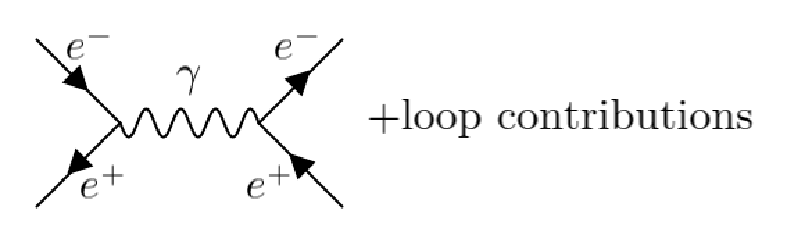
\includegraphics[]{Images/eeee.pdf}}
% In each diagram we have to put the bare coupling and renormalize to have an expression in terms of $g(E)$, where $E$ is the energy of our process. In this case, it corresponds to the exchanged momentum, $E=\sqrt{s}$. Start with the Lagrangian:
In QED, the bare Lagrangian is given by:
\[
\pazocal{L}=-\frac{1}{4}F^2_{\mu\nu}+\Bar{\Psi}^0(i\slashed{\partial}-e_0\gamma^\mu A_\mu^0-m^0)\Psi^0
\]
The quantities appearing here are infinite, the dimensions of the fields can be read off from the Lagrangian:
\[
[A_\mu^0]=\frac{d-2}{2} \quad [\Psi^0]=\frac{d-1}{1} \quad [m^0]=1 \quad [e^0]=\frac{4-d}{2}
\]
Notice that the bare charge is dimensionless only if $d=4$. We want to use \textbf{dimensional regularization}, i.e. extend the Lagrangian from 4 dimensions to $d=4-\varepsilon$ dimensions. Moreover, we would like the charge renormalized charge $e_R$ to be a number, therefore we rescale everything:\marginnote{We are using $Z_e$ instead of $Z_1$, keeping in mind that $Z_1=Z_eZ_2Z_3^{1/2}$.}
\[
A_\mu=\frac{a_\mu^0}{Z_3^{1/2}} \quad \Psi=\frac{\Psi^0}{Z_2^{1/2}} \quad m_R=\frac{m^0}{Z_m} \quad e_R=\frac{e^0}{Z_e}\mu^{\frac{d-4}{2}}
\]
which leads to:
\[
\pazocal{L}=-\frac{1}{4}Z_3F_{\mu\nu}^2+iZ_2\Bar{\Psi}\slashed{\partial}\Psi-m_RZ_2Z_m\Bar{\Psi}\Psi-\mu^{\frac{4-d}{2}}e_RZ_eZ_2Z_3^{1/2}\Bar{\Psi}\slashed{A}\Psi
\]
$Z_X=1+\delta_X$ where $\delta_X$ are the counterterms, which can be computed in the $\overline{\text{MS}}$ scheme and turn out to be:\marginnote{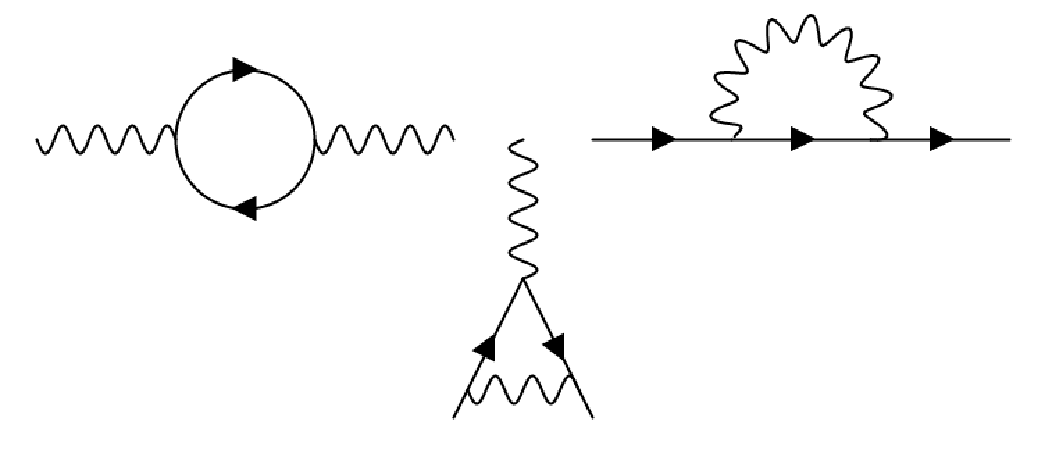
\includegraphics{Images/corrections.pdf}\\
The counterterms come from electron self-energy, photon self-energy and vertex corrections, whose diagrams are depicted above.}
\begin{align*}
\delta_2&=\frac{e_R^2}{16\pi^2}\left(-\frac{2}{\varepsilon}\right) \quad &&\delta_3=\frac{e_R^2}{16\pi^2}\left(-\frac{8}{3\varepsilon}\right)\\
\delta_m&=\frac{e_R^2}{16\pi^2}\left(-\frac{6}{\varepsilon}\right) \quad &&\delta_e=\frac{e_R^2}{16\pi^2}\left(\frac{4}{3\varepsilon}\right)
\end{align*}
Since there is $\mu$ dependence in the renormalized Lagrangian but not in the bare one, we must have:
\[
0=\mu\frac{d}{d\mu}e^0=\mu\frac{d}{d\mu}=\mu^{\frac{\varepsilon}{2}}e_RZ_e\left[\frac{\varepsilon}{2}+\frac{\mu}{e_R}\frac{de_R}{d\mu}+\frac{\mu}{Z_e}\frac{dZ_e}{d\mu}\right]
\]
At the leading order in $e_R$, $Z_e=1$ therefore:
\[
\mu\frac{de_R}{d\mu}=-\frac{\varepsilon}{2}e_R
\]
Moving to the next order, we have:
\[
\mu\frac{dZ_e}{d\mu}=\mu\frac{d}{d\mu}\left(1+\frac{e_R^2}{16\pi^2}\frac{4}{3\varepsilon}\right)=\frac{e_R}{6\varepsilon\pi^2}\mu\frac{de_R}{d\mu}=-\frac{e_R^2}{12\pi^2}
\]
where in the last step we used the relation obtained above. Finally, we get that in QED:
\[
\beta(e_R):=\mu\frac{de_R}{d\mu}=-\frac{\varepsilon}{2}e_R+\frac{e_R^3}{12\pi^2}
\]
$Z_1$ is obtained from the $\Bar{\Psi}A_\mu\Psi$ vertex, $Z_3$ from the vacuum polarization diagrams and $Z_2$ from the electron self-energy. In QED, since $Z_1=Z_2$, the $\beta$-function can be obtained from $Z_3$ alone.
% \[
% \Rightarrow\beta(g,\varepsilon):=\mu\frac{d}{d\mu}g(\mu)=\varepsilon g(\mu)-g(\mu)\frac{1}{Z_g}\mu\frac{d}{d\mu}Z_g\xrightarrow[\varepsilon\to0]{}\beta(g)
% \]
% We have to compute $Z_i$, defined as $Z_i=i+\delta_i$ with $\delta_i\sim\frac{1}{\varepsilon}g^2c_i+\dots$\\ Take now the interaction term in the Lagrangian:
% \[
% g(\mu)\mu^{-\varepsilon}\underset{\mathclap{\tikz \node {$\downarrow$} node [below=1ex] {\footnotesize $\simeq1+\delta_g+\delta_\Psi+\frac{1}{2}\delta_A:=1+\delta_V$ };}}{\underbrace{Z_gZ_A^{1/2}Z_\Psi}}\Bar{\Psi}\gamma^\mu\Psi A_\mu
% \]
% $\delta_V$ is obtained by computing the vertex correction and requiring that it cancels the divergence. We need $\delta_\Psi$ and $\delta_A$ to get $\delta_g$: computing the corrections to the electron and photon propagator, one obtains these two terms. In the $\overline{\text{MS}}$ scheme, $Z_g=1+\delta_g=1+\frac{1}{\varepsilon}g^2(\mu)c_g+\text{finite terms}$:
% \begin{align*}
% \mu\frac{d}{d\mu}Z_g&=\frac{1}{\varepsilon}c_g\mu\frac{d}{d\mu}g(\mu)^2=\frac{1}{\varepsilon}c_g2g(\mu)\mu\frac{d}{d\mu}g(\mu)\\
% &\underset{\mathclap{\tikz \node {$\uparrow$} node [below=1ex] {\footnotesize recursively};}}{=}\frac{1}{\varepsilon}c_g2g(\mu)[\varepsilon g(\mu)+\pazocal{O}(g^2)]=2c_gg(\mu)^2+\pazocal{O}(g^3)
% \end{align*}
% At this point it is possible to compute $\beta(g,\varepsilon)$:
% \begin{align*}
% \beta(g,\varepsilon)&=\varepsilon g(\mu)-2c_gg(\mu)^3+\pazocal{O}(g^4)\xrightarrow[\varepsilon\to0]{}-2c_gg(\mu)^3+\pazocal{O}(g^5)\\
% &=\frac{g^3}{12\pi^2}+\pazocal{O}(g^5)
% \end{align*}
\end{example}
As we have just seen, in QED the $\beta$-function is positive, this means that the interaction coupling grows with the energy. In principle, one can imagine scattering processes at arbitrary high energies where the coupling will explode: QED is not a complete theory, it does not work at arbitrary high energies.\\
Usually, we stop at first order in the $\beta$-function because the coupling is small, but as it gets bigger we have to include higher order terms too. By including higher order terms, theory may \textit{cure itself}, for example with a change of sign. In this case, for a certain value of the coupling $g$, denoted by $g^*$, the theory does not evolve anymore and the coupling constant is really a constant. At this so-called \textbf{fixed point}, the theory is \textbf{conformal}, there is no physical scale and everything is invariant. Sadly, this fixed point does not exist in QED, so the theory explodes at some point and it has to be replaced by something else. This is what we call an \textbf{effective theory}, a theory valid only at low energy that has to be replaced with another theory which guarantees a more fundamental description. This is what we do by introducing the \textbf{Standard Model}.\\
QED is an abelian gauge theory, for non-abelian gauge theories, we have to take into account more 1-loop contributions than the abelian case.\marginnote{For example, in QCD gluons are self-interacting.} By doing so, at 1-loop one founds:
\begin{equation}
\labeq{beta0}
\beta_0=-\frac{11}{3}C_2(\text{adj})+\frac{4}{3}T(r_f)n_f+\frac{1}{3}T(r_s)n_s
\end{equation}
$C_2$ is the quadratic Casimir of the adjoint representation, $T(n_f)$ is the \href{https://en.wikipedia.org/wiki/Eugene_Dynkin}{Dynkin} index for a certain representation of fermions, $n_f$ denotes the number of fermions, $T(r_s)n_s$ is the same thing as the fermions but with complex scalars.\\
The first term is negative, if we do not have too many matter fields, this will be the dominant one and the $\beta$-function will be negative, so as the energy increases the coupling decreases. It is therefore possible to extrapolate the theory at arbitrary high energies, this is called \textbf{asymptotic freedom}\marginnote{Asymptotic freedom explains a number of important qualitative features of the strong interaction, such as how QCD can be strong but also short-ranged and why free quarks have never been seen}. On the other hand, at low energies the coupling will increase and we cannot treat the theory perturbatively anymore.\\
Specializing now to QCD with $N_c=3$ and $n_f=6$. In this case, \refeq{beta0} tells us that:
\[
\beta_0=-\frac{11}{3}N_c+\frac{2}{3}n_f=-7<0
\]
% As long as there are less than 17 flavours of quarks (there are six in nature), $\beta_0<0$ hence $g(\mu)$ decreases with increasing $\mu$. Compare this result with the one for the abelian case, where we have:
% \[
% \beta_0=\frac{4}{3}q^2_\Psi n_f+\frac{1}{3}q_s^2n_s
% \]
% Here the first term of the non-abelian case is not present because there is no self-interaction and $\beta_0$ is always larger than zero, while in the non-abelian case it depends on the number of fermions and scalars.\\
In the abelian case, the coupling evolves until it becomes zero for $E\to0$. The variation of velocity is zero, there is no evolution and this is reached only asymptotically. Conversely, when the energy increases the $\beta$-function increases too and we have two possibilities as $E\to\infty$: 
\begin{enumerate}
    \item $\beta(g)$ remains positive and there are two sub-cases: $g(E)\to\infty$ for $E\toE_0$ (\href{https://en.wikipedia.org/wiki/Lev_Landau}{Landau} pole) or $g(E)\to\infty$ as $E\to\infty$. In both cases, the theory is not complete.
    \item $\beta$ function has a zero for some finite value $g^*$ called UV fixed point. The theory does not evolve anymore once it reaches this fixed point, which is possible only asymptotically.
\end{enumerate}
As anticipated, in QED we encounter the first case.\marginnote{From \cite{schwartz}, Section 23.2.} We are going to look at it more in detail now. From previous calculations, we know that, neglecting the contribution of higher order terms, we have:
\begin{equation}
\labeq{betaqed}
\beta(e_R)=\mu\frac{de_R}{d\mu}=-\frac{\varepsilon}{2}e_R+\frac{e_R^3}{12\pi^2}
\end{equation}
Sometimes, this is written as a function of $\alpha=\frac{e_R^2}{4\pi}$, which gives us:
\[
\beta(\alpha):=\mu\frac{d\alpha}{d\mu}=\frac{e_R}{2\pi}\mu\frac{de_R}{d\mu}=-\frac{\varepsilon}{4\pi}e_R^2+\frac{e_R^4}{24\pi^3}+\dots=-\varepsilon\alpha+\frac{2}{3\pi}\alpha^2+\dots
\]
Conventionally, this expansion is written as:
\[
\beta(\alpha)=-2\alpha\left[\frac{\varepsilon}{2}+\left(\frac{\alpha}{4\pi}\right)\beta_0+\left(\frac{\alpha}{4\pi}\right)^2\beta_1+\dots\right]
\]
Matching the result in \refeq{betaqed} gives us $\beta_0=-\frac{4}{3}$, at the leading order and at $\varepsilon=0$ we can solve this equation:
\[
\mu\frac{d\alpha}{d\mu}=\frac{2}{3\pi}\alpha^2\to\int_{\alpha(\mu)}^{\alpha(M)}\frac{d\alpha}{\alpha^2}=\frac{2}{3\pi}\int_\mu^M\frac{d\mu}{\mu}
\]
where $M$ is a certain scale. Computing the integral gives us:
\[
\frac{1}{\alpha(\mu)}-\frac{1}{\alpha(M)}=\frac{4\pi}{e_R^2(\mu)}-\frac{4\pi}{e_R^2(M)}=\frac{2}{3\pi}\ln{(M/\mu)}=\frac{\beta_0}{2\pi}\ln{(\mu/M)}
\]
This tells us that:
\[
\frac{1}{e_R^2(\mu)}=\frac{1}{e_R^2(M)}+\frac{2\beta_0}{16\pi^2}\ln(\mu/M)\Rightarrow e_R^2(\mu)=\frac{e_R^2(M)}{1+\frac{\beta_0}{16\pi^2}e_R^2(M)\ln(\mu^2/M^2)}
\]
We check that it has the right behaviour:
\begin{itemize}
    \item for $\mu<M, \mu\to0$: $e_R(\mu)\to0$, the dominating term is the logarithmic one.
    \[
    e_R^2(\mu)\approx\frac{16\pi^2}{\beta_0}\frac{1}{\ln(M^2/\mu^2)}
    \]
    \item for $\mu=M$, $e_R^2(\mu)=e_R^2(M)$
    \item for $\mu>M$, the denominator will be smaller than 1 and the coupling will increase. There will be a Landau pole, denoted by $\Lambda_{\text{QED}}$:
    \[
    1+\frac{\beta_0}{16\pi^2}e_R^2(M)\ln(\mu^2/M^2)=0\to\Lambda_{\text{QED}}:=M\exp{-\frac{8\pi^2}{\beta_0}\frac{1}{e_R^2(M)}}
    \]
\end{itemize}
Using $\alpha(m_e=511\,\text{keV})=\frac{e_R^2(m_e)}{4\pi}=\frac{1}{137}$, we find $\Lambda_{\text{QED}}=10^{286}$\,eV. In doing this, we swapped a dimensionless number for a dimensionful scale: this is known as \textbf{dimensional transmutation}. This uncovers a very profound misconception about nature: electrodynamics is fundamentally defined not by the electric charge, as we learned classically, but by a dimensionful scale $\Lambda_{\text{QED}}$. Moreover, this scale only has a meaning if there is another scale in the theory, such as the electron mass, so really it is the ratio $m_e/\Lambda_{\text{QED}}$ which specifies QED completely.\\
We cannot use perturbation theory anymore because the coupling becomes too large. If we want to reach the IR fixed point there will be other scales, because we reach a point where energies are compatible with the mass of the electron. Electrons contribution in the diagram will be cancelled for energies smaller than the mass of the electron, so we can create an effective theory without electrons, cutting it off and this theory has only the photon with some self-interaction reduced by virtual electrons loops. These interactions disappear at low energies but at this point is not QED anymore, it is a theory of only photons.\\
At the fixed points of the renormalization groups $\beta(g)=0$: $g$ is a constant, the theory, without mass, is self-similar. In a normal situation, by changing the energy we obtain different results for scattering processes because we have running coupling, while in this case we have the same results because the theory does not evolve anymore. Scattering processes do not depend anymore on the energy of the particles involved.\\
\underline{QED for $m_e=0$}:
\[
\pazocal{L}=-\frac{1}{4}F_{\mu\nu}^2+\Bar{\Psi}\gamma^\mu i(\partial_\mu-igA_\mu)\Psi
\]
This Lagrangian does not contain scales, it is invariant under change of scale at the classical level. When we include corrections, the coupling evolves because the renormalization process includes a scale factor ($\mu$) and this scale evolves. Once the fixed points are reached, we are back in a situation analogous to the classical one: the theory does not evolve anymore, hence it is invariant under scale change. Theories with UV fixed points are called \textbf{asymptotically safe}. Asymptotic safety is a generalization of asymptotic freedom: with asymptotic freedom the coupling goes to zero, while with asymptotic safety the coupling goes to a certain finite constant. Is QED asymptotically safe? No,the fixed points can be reached for small values of the coupling, where we can use perturbation theory to find $g^*$ but computations show that this point does not exist. Another possibility is to have $g*$ for large values of the coupling, where we cannot use perturbation theory and again this fixed point does not exist. QED is an \textbf{effective field theory}, it explodes at some point.\\
\underline{Non-abelian gauge theories SU$(N)$ (QCD)}: in the non-abelian case, it can happen to have so many massless flavours that the $\beta_0$ contribution in the $\beta-$function coming from the matter is bigger than the negative contribution coming from the gauge field, resulting in $\beta_0>0$. However, we do not have only one gauge field, but $N^2-1$ fields. For simplicity, consider only fermions in the fundamental representation:\marginnote{It is the same thing for scalars.}
\[
\beta_0=-\frac{11}{3}N+\frac{2}{3}n_f\to\beta_0>0 \;\text{for}\;n_f>\frac{11}{2}N
\]
The theory is in the non-abelian Coulomb phase. Decreasing $n_f$ results in $\beta_0<0$:
\[
\beta(g)=\frac{\beta_0}{16\pi^2}g^3+\frac{\beta_1}{(16\pi^2)^2}g^5+\dots
\]
At some point, there can be a cancellation between the two terms:
\[
\beta(g^*)=0 \;\text{for}\;\frac{g^*^2}{16\pi^2}\beta_1=|\beta_0|
\]
Can we trust this calculation if there are higher order terms in $\beta(g)$? We can neglect terms of order $>g^5$ if we choose a value of $n_f$ below but close to the threshold, $n_f<11N/2$. This computation is reliable for $|\beta_0|/\beta_1\ll1$, i.e. $N,n_f\gg1$ but $n_f/N\lesssim11/2$. In UV, the theory is asymptotically free, because increasing $E$ results in $\beta_0<0$ and the coupling goes to zero. If we decrease the number of flavours $n_f$, $|\beta_0|$ increases and $g^*$ gets larger: there is a value $n_f^c$ below which there is no IR fixed point. If the number of flavours $n_f$ is kept between $n_f^c$ and $11N/2$, we are in the \textbf{conformal window} and there exists an IR fixed point. For $n_f=n_f^c$ we have one critical point, but if we below this critical value the coupling gets bigger and bigger and eventually it explodes. This tells us that we have to take into account some non-perturbative contribution. QCD is a theory of this type where there is confinement for $n_f\in(0,n_f^c)$: this confinement space is characterized by the presence of bound states. The coupling gets so big that we have the formation of non-perturbative bound states called \textbf{hadrons}. They are not states like the hydrogen atom, they are made by fermions and gauge fields together and are colour singlet, i.e. they form singlets of SU$(N)$. Colour does not appear at large distance (small energy). The Lagrangian is written in the UV range, hence at extremely high energies where the theory is perturbative, but when we go to lower energies the phenomenology is completely different.\\
What kind of bound states can we have?
\begin{itemize}
    \item \textbf{Baryons}: made only of quarks, we take $N$ quarks and contract them with an $\varepsilon$ tensor. In the case of QCD, $N=3$.
    \item \textbf{Mesons}: made of one quark $q$ and an anti-quark $\Bar{q}$, $\Bar{q}_iq^i=\Bar{q}_jq^i\delta_i^j$\marginnote{There are also other possibilities like tetra- and penta-quarks but they are exotic states. We know they are resonances so they have a short lifetime.}
\end{itemize}
At which scale are these bound states created? We can make a simple estimate by solving the running coupling equation at 1-loop:
\[
g^2(\mu)=\frac{g^2(M)}{1-\frac{\beta_0}{16\pi^2}g^2(M)\log(\mu^2/M^2)}\Rightarrow\Lambda=M\exp{-\frac{8\pi^2}{\beta_0}\frac{1}{g^2(M)}}
\]
$M$ denotes the energy at which we can measure the coupling, we decrease it until we reach a value $\Lambda$ where the coupling explodes. The expression for $g^2(\mu)$ holds true only when the coupling is small, but it gives us an idea of the value of the energy at which the coupling becomes non-perturbative.

Classically, we start from a theory where we do not have any dimensional parameter, just the kinetic term for the gauge fields and the massless fermions:
\[
\pazocal{L}=-\frac{1}{4}(F_{\mu\nu}^a)^2+\sum_{i=1}^{n_f}\Bar{\Psi}_ii\slashed{D}\Psi_i
\]
The action is invariant since there are no dimensional parameter, so there is nothing fixing a reference scale. However, this is valid only on a classical level: in the Lagrangian, there is the coupling in the covariant derivative and in the non-abelian interaction term, so these parameters are dimensionless but we have seen that the coupling introduces a scale $\Lambda$. This phenomenon is called \textbf{dimensional transmutation}: starting from a theory with only dimensionless parameters we arrive to a theory which has an intrinsic scale due to coupling when it gets non-perturbative, $\Lambda$ is generated dynamically from the theory.\marginnote[-3.5cm]{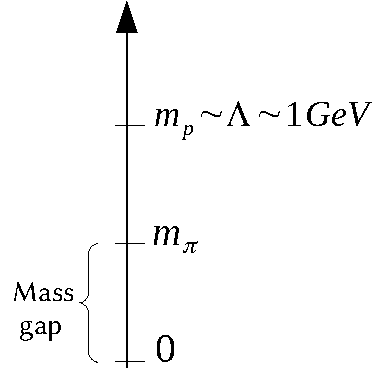
\includegraphics[]{Images/massgap.pdf}} $\Lambda$ fixes the mass gap, except for lightest bound states ($m_\pi$) which arise from spontaneous symmetry breaking and they will be treated as pseudo-Nambu-Goldstone bosons.\\
We have seen that a possibility for the $\beta-$function is to have an IR fixed point which appears in vectorial SU$(N)$ gauge theories with $n_f$ Dirac fermions. The possibility to have this perturbative IR fixed point requires $n_f\lesssim11N/2$. What happens if we consider instead massive fermions? When we decrease the energy, we start inside the conformal window so the coupling will move towards the fixed point. 
\begin{figure}[h]
    \centering
    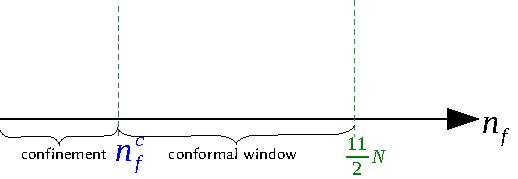
\includegraphics{Images/conf.pdf}
    \caption*{}
    \label{fig:my_label}
\end{figure}
At some point, we will get to the energy of the order of the mass of the first fermion, $E\sim m_{f_1}$, and the contribution of any Feynman diagram coming from the virtual propagation of this fermion will freeze. Going to energies below $m_{f_1}$, we can forget about this fermion and write an effective theory without considering it. Repeating this argument for more fermions, we may find ourselves outside the conformal window and enter the confinement phase, where there will be a threshold at which bound states are formed, i.e. the dynamical scale $\Lambda$. In principle, there could be also other fermions lighter than $\Lambda$ which do not necessarily have to be massless (this is the case of QCD). All the lighter fermions behave as if they were massless even if they are not and the number of these fermions tells us where we are in the graphic above. In QCD, there are 3 lighter fermions (up, down and strange), the dynamical scale $\Lambda\approx(100\text{MeV}-1\text{GeV})$ (charm) and two heavier fermions (top and bottom).
\section{Spin-1 Particle as a Gauge Theory}
Consider the \href{https://en.wikipedia.org/wiki/Alexandru_Proca}{Proca} Lagrangian for massive spin-1 particles:
\[
\pazocal{L}_p=-\frac{1}{4}V_{\mu\nu}^2+\frac{m_v^2}{2}V_\mu^2 \quad V_{\mu\nu}=\partial_\mu V_\nu-\partial_\nu V_\mu
\]
We want to understand how this Lagrangian is connected with gauge invariance and gauge symmetry. To do that, we use the so-called \href{https://en.wikipedia.org/wiki/Ernst_Stueckelberg}{Stueckelberg} trick which is nothing but a change of variables in which we put $V_\mu(x)=A_\mu(x)-\partial_\mu\pi(x)$, where $A_\mu(x)$ is a gauge field and $\pi(x)$  a scalar field. This description is not unique, we can choose the two fields in different ways. We have a redundancy, with these new variables, the Lagrangian is invariant under:
\[
\left\{
\begin{aligned}
&A_\mu(x)\to A_\mu(x)+\partial_\mu\varepsilon(x)\\
&\pi(x)\to\pi(x)+\varepsilon(x)
\end{aligned}
\right.
\]
We are adding one more degree of freedom at the cost of having this redundancy.\marginnote{Basically because we do not need another degree of freedom, we could set $\pi(x)=0$ and get back to the initial case.} In terms of the new variables, the Proca Lagrangian becomes:
\[
\pazocal{L}_p=-\frac{1}{4}F_{\mu\nu}^2+\frac{m_v^2}{2}(A_\mu(x)-\partial_\mu\pi(x))^2=-\frac{1}{4}F_{\mu\nu}^2+\frac{m_v^2}{2}A^2_\mu+\frac{m_v^2}{2}(\partial_\mu\pi)^2-m_v^2A_\mu\partial_\mu\pi
\]
The last term mixes $A_\mu$ and $\pi$ and we want to eliminate it. We can exploit the redundancy and choose the new terms such that this term vanishes.\marginnote{For example, we can remove it assuming $\partial_\mu A_\mu=0$. This is a possible choice, but we are not going to use it.} We introduce a gauge-fixing Lagrangian to cancel that term:
\[
\pazocal{L}_{GF}=-\frac{1}{\xi}(\partial_\mu A^\mu+\xi m_v^2\pi)^2=-\frac{1}{2\xi}(\partial_\mu A^\mu)^2-\frac{1}{2}\xi m_v^4\pi^2-m_v^2\partial_\mu A^\mu\pi
\marginnote{A me sembra che stiamo gauge-fixando una beata sega ma tant'è.}
\]
$\xi$ is an arbitrary dimensionless parameter, we define $\chi(x):=m_v\pi(x)$ and write everything as:
\[
\pazocal{L}=\pazocal{L}_p+\pazocal{L}_{GF}=-\frac{1}{4}F_{\mu\nu}^2+\frac{m_v^2}{2}A_\mu^2-\frac{1}{2\xi}(\partial_\mu A^\mu)^2+\frac{1}{2}(\partial_\mu\chi)^2-\frac{1}{2}\xi m_v^2\chi^2
\]
This is now the Lagrangian of our theory with no mixed terms. The first part resembles a gauge theory, except for the mass term which seems a bit odd, while the second part is a scalar theory. In order to quantize the theory, we can invert the kinetic term to get the propagator so that we can understand how many physical degrees of freedom are there: we started with 3 degrees of freedom and now apparently we have 4 of them. We have to study the poles of the propagators.
\begin{itemize}
    \item $A_\mu$ propagator:
    \[
    \Pi_{\mu\nu}(p)=\frac{-i}{p^2-m_v^2}\left[\eta_{\mu\nu}+(\xi-1)\frac{P_\mu P_\nu}{p^2-\xi m_v^2}\right]
    \]
    It has two poles, an expected one in $p^2=m_v^2$ and an unexpected on in $p^2=\xi m_v^2$ which is unphysical.
    \item $\chi$ propagator:
    \[
    \Pi(p)=\frac{i}{p^2-\xi m_v^2}
    \]
    $\xi$ is an arbitrary parameter, the physics cannot depend on it. This pole has to vanish somehow: the propagation of $\chi$ cancels the non-physical quantity in the gauge field propagator. 
\end{itemize}
$\chi$ itself is not a physical quantity, there are only the three degrees of freedom from the propagator of $A_\mu$ which is the only one to have a physical pole. It is useful to rewrite $\Pi_{\mu\nu}(p)$ in the following way:
\[
\Pi_{\mu\nu}(p)=\underbrace{\frac{-i}{p^2-m_v^2}\left[\eta_{\mu\nu}-\frac{P_\mu P_\nu}{m_v^2}\right]}_{\text{massive spin-1 particle propagator}}-\underbrace{\frac{i}{p^2-\xi m_v^2}\frac{P_\mu P_\nu}{m_v^2}}_{\text{unphysical content}}
\]
The gauge-fixing we introduced is called the $\xi-$gauge, this kind of gauges are good to test the renormalization of massive spin-1 field theories. When we do renormalization, we want to see what are the diagrams which diverge, because if we have a finite number of diverging diagrams we can renormalize the theory by introducing a finite number of counter-terms. In the propagator of a massive spin-1 particle, if we take the limit $p\to\infty$ there is a term going as $1/p^2$ and one which goes as $p^2$, so the propagator goes as $p^0$. This is obviously not good, because it means there is a possibility that when doing the diagrams all of them are divergent and the theory is not renormalizable. Luckily, this is not our case, we are going to see that this Lagrangian can be brought back to a gauge theory, even if we have that odd mass term for the moment.\\
We can make another redefinition of the field before adding the gauge-fixing term:
\[
\frac{1}{2}(\partial_\mu\chi-m_vA_\mu)^2=\frac{1}{2}\frac{1}{v^2}\left|\left(\partial_\mu-i\frac{m_v}{v}A_\mu\right)e^{i\chi/v}\right|^2
\]
with $v$ an arbitrary parameter introduced to have an dimensionless argument in the exponential. This is the mass term, we define the coupling $g:=m_v/v$: in terms of mass, both terms have dimension 1 but if we add $\hbar$ they have different dimensions because the coupling is not dimensionless in $\hbar$.
\[
\alpha=\frac{e^2}{4\pi\hbar c} \;\text{dimensionless}\Rightarrow[e^2]_\hbar=1/2
\]
\begin{example} We make an example to verify the dimensionality of things.
\begin{align*}
&\frac{S}{\hbar}=\frac{1}{\hbar}\int d^4x\pazocal{L}(\phi,\partial_\mu\phi)\\
&\pazocal{L}(\phi,\partial_\mu\phi)=\frac{1}{2}(\partial_\mu\phi)^2-\frac{m^2}{2}\phi^2+\lambda_3m\phi^3+\lambda_4\phi^4+\dots
\end{align*}
To get rid of $\hbar$, we can redefine the field as $\phi\to\phi:=\phi'\hbar^{1/2}$.
\[
\frac{S}{\hbar}\to\int d^4x\left[\frac{1}{2}(\partial_\mu\phi)^2-\frac{m^2}{2}\phi^2+\lambda_3m\hbar^{1/2}\phi^3+\lambda_4\hbar\phi^4+\dots\right]
\]
The n-th term will go as $\hbar^{(n-2)/2}\lambda_n\phi^n$ and it is possible to define $\lamda_3m\hbar$ and $\lambda_4\hbar$ so that they go as a coupling, i.e. with dimension 1/2 in terms of $\hbar$. For example, if we want to see the expansion parameter in a perturbative series it will be coupling$^2$/$(4\pi)^2$, every time we introduce a new order in the series we add a power of $\hbar$. In other words, the expansion in a perturbative series is nothing but a series of powers of $\hbar$. If we have an observable $A$, it is possible to write it as:
\[
A=a_0+a_1\hbar+a_2\hbar^2+\dots \quad a_n\sim\left(\frac{\text{coupling}^2}{(4\pi)^2}\right)^n
\]
From the initial redefinition of the field, we have that $[\phi']=-1/2$ since $\phi$ is dimensionless, while if we look at the vacuum expectation value (vev), $\langle\phi\rangle=v$ and $[v]_\hbar=-1/2$. The physical mass is dimensionless in $\hbar$, it has nothing to do with it hence it follows that:
\[
[g]_\hbar=\frac{[m_v]_\hbar}{[v]_\hbar}\Rightarrow[g]_\hbar=1/2
\]
\end{example}
Let's get back to our initial calculation and define a new field $\varphi(x):=ve^{i\chi(x)/v}$, the mass term can be written as:
\[
\frac{1}{2}m_v^2V_\mu V^\mu=\frac{1}{2}|D_\mu\varphi|^2 \quad D_\mu=\partial_\mu-igA_\mu
\]
This is something familiar now: the mass term becomes the kinetic term for the field $\varphi$. The Lagrangian gets now written in the following way:
\[
\pazocal{L}=-\frac{1}{4}F_{\mu\nu}^2+\frac{1}{2}|D_\mu\varphi|^2-\frac{1}{2\xi}(\partial_\mu A^\mu+\xi gv\mathfrak{Im}\varphi)^2
\]
This is now a gauge theory in which the fields transform like:
\[
\left\{
\begin{aligned}
&\chi(x)\to\chi(x)+m_v\varepsilon(x)\\
&\varphi(x)\toe^{im_v\varepsilon(x)/v}\varphi(x)=e^{ig\varepsilon(x)}\varphi(x)\\
&A_\mu(x)\to A_\mu(x)+\partial_\mu\varepsilon(x)
\end{aligned}
\right.
\]
By defining $\alpha(x):=g\varepsilon(x)$ it becomes a gauge transformation which acts linearly. Before it was not a linear transformation in $\chi$ because there was a non-linear shift, moreover $\varphi$ is subject to a non-linear constraint $\varphi^\dagger\varphi=v^2$.\\
At this point, we forget about all the considerations we made about gauge transformations and we consider U(1):$\varphi(x)\to e^{i\alpha(x)}\varphi(x)$. We have a gauge theory with a U(1) global symmetry non-linearly realized, $\chi$ is nothing but the NGB corresponding to this spontaneously broken global invariance: this symmetry is not realized à la Wigner, but rather à la Nambu-Goldstone.

\section{\href{https://en.wikipedia.org/wiki/Robert_Brout}{Brout}-\href{https://en.wikipedia.org/wiki/Francois_Englert}{Englert}-\href{https://en.wikipedia.org/wiki/Peter_Higgs}{Higgs} Mechanism}

Spontaneous Symmetry Breaking (SSB) does not occur when we have a potential, here for example we do not have one. The important thing is how this symmetry is realized, whether à la Wigner (linearly) or à la Nambu-Goldstone (non-linearly). It is the global invariance to be broken, not the gauge one which is a redundancy and cannot be spontaneously broken. If we go to energies much larger than the mass of this spin-1 particle, then we can ignore it. Our theory has 3 degrees of freedom, which are the three possible polarizations $(\sigma=-1,0,+1)$: at high energies we can include the theory in the Poincaré group and treat it as a massless spin-1 particle plus a scalar. So it is a gauge theory both at high energies and at low energies since we have SSB. We neglect the mass term for $E\gg m_v$:
\[
\pazocal{L}=\underbrace{-\frac{1}{4}F_{\mu\nu}^2-\frac{1}{2\xi}(\partial_\mu A_\mu)^2}_{\text{massless spin-1 particle}}+\underbrace{\frac{1}{2}(\partial_\mu chi)^2}_{\text{scalar}}
\]
The scalar acts as the longitudinal polarization of a massive spin-1 particle: at high energies it is described by the Goldstone boson which becomes physical when we go to extremely high energies. It is important to separate these degrees of freedom because, as we are going to see, they behave in completely different ways.\\
At this point we want to get rid of the constraint $\varphi^\dagger\varphi=v^2$ and we can show that in order to do that we have to introduce another degree of freedom, another scalar: the \textbf{Higgs boson}. We start with:
\[
\pazocal{L}=-\frac{1}{4}F_{\mu\nu}^2+|D_\mu\varphi|^2-V(\varphi) \quad V(\varphi)=-\mu^2(\varphi^\dagger\varphi)+\lambda(\varphi^\dagger\varphi)^2
\]
We had to introduce a potential for $\varphi$, the so-called Mexican hat potential.
\begin{figure}[h]
    \centering
    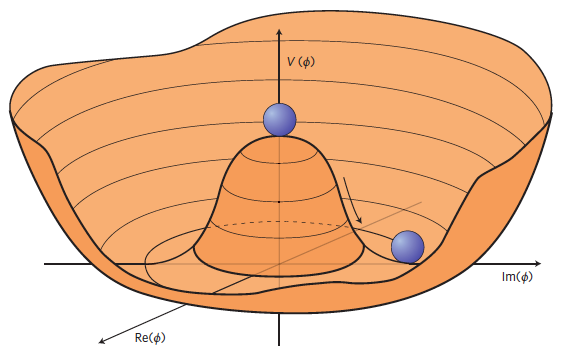
\includegraphics{Images/higgspotential.png}
    \caption{Mexican hat potential.}
    \label{fig:my_label}
\end{figure}\\
We want to spontaneously break the U(1) invariance, so the mass term $-\mu^2$ has to be negative. The vacuum expectation value (vev) is $\langle\varphi\rangle=v/\sqrt{2}$, substituting this expression in the potential and minimizing it we find $v^2=\mu^2/\lambda$. We can parameterize our field $\varphi(x)$ by using another field $\eta(x)$:
\[
\varphi(x)=\frac{v+\eta(x)}{\sqrt{2}}e^{i\chi(x)/v}
\]
corresponding to the vev+fluctuation given by $\eta(x)$. There are two types of possible excitations:
\begin{itemize}
    \item \textbf{angular} excitation around the valley of minima. This excitation is described by $\chi(x)$ giving massless NGB since we are moving around the valley of minima.
    \item \textbf{radial} excitation changing the distance from the origin. It will be massive, resulting in the Higgs boson, the extra degree of freedom we added.
\end{itemize}
We can write the Lagrangian in terms of this new $\varphi(x)$, adding the gauge-fixing part to get rid of the mixing terms arising from the covariant derivative. What we will obtain is the same Lagrangian as before plus $\eta(x)$ terms which can be removed by taking $\mu^2,\lambda\to\infty$ so that $v$ is fixed and we get back to the non-linear expression we had before.\\
We want to take a closer look at the kinetic term in $\varphi$:
\begin{align*}
D_\mu\varphi&=\frac{1}{\sqrt{2}}(\partial_\mu-igA_\mu)(v+\eta)e^{i\chi/v}\\
&=\frac{1}{\sqrt{2}}\left[\partial_\mu\eta e^{i\chi/v}+(v+\eta)i\frac{\partial_\mu\chi}{v}e^{i\chi/v}-igA_\mu(v+\eta)e^{i\chi/v}\right]\\
&=\frac{e^{i\chi/v}}{\sqrt{2}}\left[\partial_\mu\eta+i\left(\frac{\partial_\mu\chi}{v}-gA_\mu\right)(v+\eta)\right]
\end{align*}
We take the modulus squared of this object and we are left with:
\[
|D_\mu\varphi|^2=\frac{1}{2}\left[(\partial_\mu\eta)+\left(1+\frac{\eta}{v}\right)^2(\partial_\mu\chi-gvA_\mu)^2\right]
\]
When expanding the square in the last term, we obtain a mixing term which we want to get rid of. Again, we add a gauge-fixing term to remove this unwanted part:
\[
\pazocal{L}_{GF}=-\frac{1}{2\xi}(\partial_\mu A^\mu+\xi gv\chi)^2
\]
We define $m_A:=gv$ and write:
\[
\pazocal{L}+\pazocal{L}_{GF}=-\frac{1}{4}F_{\mu\nu}^2-\frac{1}{2\xi}(\partial_\mu A^\mu)^2+\frac{1}{2}(\partial_\mu\chi)^2\left(1+\frac{\eta}{v}\right)^2-\frac{1}{2}\xi m_A^2\chi^2+\frac{1}{2}m_A^2A_\mu A^\mu\left(1+\frac{\eta}{v}\right)^2-m_AA_\mu\partial_\mu\chi\left(\frac{2\eta}{v}+\frac{\eta^2}{v^2}\right)
\]
The Lagrangian now is no longer free, moreover we observe that:
\begin{itemize}
    \item $\chi$ interacts only through derivatives, which is good for NGB \raisebox{-\mydepth}{{
\includegraphics[height=1.1\baselineskip]{Images/smile.jpg}}}
    \item $\chi$ is massless for $\xi=0$
    \item it is possible to show that $\chi$ is an unphysical quantity (due to BRST quantization)
\end{itemize}
We now take a look at some possible choices for $\xi$:
\begin{enumerate}
    \item $\xi=1$, this is the Feynman gauge.
    \[
    \Pi_{\mu\nu}(p)=-\frac{i\eta_{\mu\nu}}{p^2-m_A^2}
    \]
    \item $\xi=0$, this is the Landau gauge.
    \[
    \Pi_{\mu\nu}(p)=-\frac{i}{p^2-m_A^2}\left(\eta_{\mu\nu}-\frac{P_\mu P_\nu}{p^2}\right)
    \]
    It is the transverse propagator, in this gauge we have $m_\chi^2=\xi m_A^2=\xi g^2v^20$ hence it is a non-physical quantity since its mass depends on an arbitrary parameter.
    \item $\xi\to\infty$, this is the unitary gauge. Before adding the gauge-fixing term, we can make a gauge transformation:
    \[
    \frac{\chi}{v}\to\frac{\chi}{v}+\alpha(x) \quad \alpha(x)=-\frac{\chi}{v} 
    \]
    We send the NGB to zero but if $\xi\to\infty$, then the mass of the NGB goes to infinity too so we cannot excite this state anymore because it would require an infinite amount of energy.
    \[
    \Pi_{\mu\nu}(p)=-\frac{i}{p^2-m_A^2}\left(\eta_{\mu\nu}-\frac{P_\mu P_\nu}{m_A^2}\right)
    \]
\end{enumerate}
The generic expression for the propagator is given by:
\[
\Pi_{\mu\nu}(p)=-\frac{i}{p^2-m_A^2}\left[\eta_{\mu\nu}+(\xi-1)\frac{P_\mu P_\nu}{p^2-\xi m_A^2}\right]
\]
In some gauges, the NGB is not present while we find it in some other ones, whether it is massive or massless. However, the Goldstone theorem [\ref{GT}] tells us that whenever we have SSB we should have a massless NGB. It seems like this theorem holds true for some cases and in some other ones it is not valid anymore: the validity of the Goldstone theorem depends on the gauge-fixing. For example, non-covariant gauges (like the Coulomb one) violate the theorem. At some point in the theory we want to prove that:
\[
\lim_{V\to\infty}[Q_V(t),\phi(0)]=\lim_{V\to\infty}\int_Vd^3x[J^0(\Vec{x},t),\phi(0)]<\infty
\]
To prove that we used microcausality, which exploits Lorentz covariance. If we work in a gauge with no Lorentz covariance, we will have some problems in this step. Even when this NGB are massless and present in the theory, they are not physical quantities. Therefore, even when the theorem is valid it does not produce a physical contribution. We can prove that by considering the fact that the $S$-matrix must be unitary when we include the physical states. Restricting the $S$-matrix to the space of physical states, without including the NGBs, keeps the $S$-matrix unitary: in a gauge theory, the NGB is never physical and we can always choose a gauge in which it is not even present.\\
For the unitary gauge, we can evaluate the spectrum starting from the Lagrangian:
\[
\pazocal{L}=-\frac{1}{4}F_{\mu\nu}^2+\frac{1}{2}m_A^2A_\mu A^\mu\left(1+\frac{\eta}{v}\right)^2+\frac{1}{2}(\partial_\mu\eta)^2-V(\eta)
\]
We observe that the physical degrees of freedom are the 3 polarizations of massive spin-1 particles+spin-0 particle $(\eta)$, resulting in 4 degrees of freedom.\marginnote{We could have observed it also from the starting Lagrangian but we would not have been able to connect it to physical states, while it is clear in the unitary gauge.}
\section{Equivalence Theorem}
\labsec{eqthm}
\begin{theorem}
The scattering amplitude of the $S$-matrix for the emission or absorption of a longitudinally polarized vector boson becomes equal, at $E\gg m_A$, to the scattering amplitude of the corresponding NGB computed in the $\xi$-gauge.
\end{theorem}
Graphically, we can see it as:
\begin{figure}[h]
    \centering
    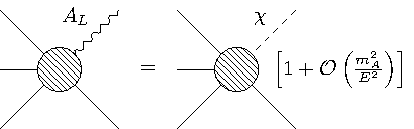
\includegraphics{Images/eqthm.pdf}
    \caption*{}
    \label{fig:my_label}
\end{figure}\\
Sometimes it is more convenient to do this type of computations with $\chi$ rather than using $A_L$. To make things clear, let's make an example: consider the scattering $A_LA_L\to A_LA_L$ and compare the two amplitudes, $M(A_LA_L\to A_LA_L)$ with $M(\chi\chi\to\chi\chi)$.   
In the unitary gauge, the Lagrangian contains:
\[
\pazocal{L}\supset\frac{m_A^2}{2}A_\mu A^\mu\left(1+\frac{\eta}{v}\right)^2=\frac{m_A^2}{v}A_\mu A^\mu\eta+\dots
\]
For this process we have 3 diagrams because there are 4 identical particles in the initial and final states.
\begin{figure}[h]
    \centering
    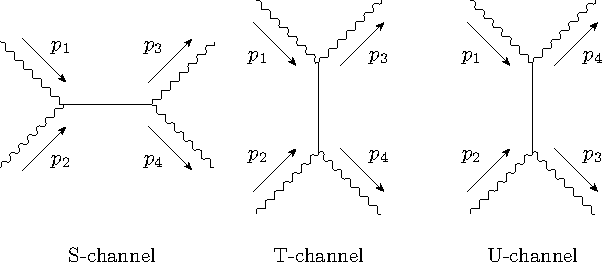
\includegraphics{Images/stu.pdf}
    \caption*{}
    \label{fig:my_label}
\end{figure}\\
We then have $M(A_LA_L\to A_LA_L)=i^2\cdot4\cdot2/2!(M_S+M_T+M_U)$, so we compute the three amplitudes:
\begin{itemize}
    \item $M_S=\left(\frac{m_A^2}{v}\right)^2\frac{i}{(p_1+p_2)^2-m_\eta^2}\varepsilon_L(p_1)\cdot\varepsilon_L(p_2)\varepsilon_L(p_3)\cdot\varepsilon_L(p_4)$
    \item $M_T=\left(\frac{m_A^2}{v}\right)^2\frac{i}{(p_1-p_3)^2-m_\eta^2}\varepsilon_L(p_1)\cdot\varepsilon_L(p_3)\varepsilon_L(p_2)\cdot\varepsilon_L(p_4)$
    \item $M_V=\left(\frac{m_A^2}{v}\right)^2\frac{i}{(p_1-p_4)^2-m_\eta^2}\varepsilon_L(p_1)\cdot\varepsilon_L(p_4)\varepsilon_L(p_2)\cdot\varepsilon_L(p_3)$
\end{itemize}
Putting everything together we obtain:
\[
M=-4i\left(\frac{m_A^4}{v^2}\right)\left[\frac{\varepsilon_L(p_1)\cdot\varepsilon_L(p_2)\varepsilon_L(p_3)\cdot\varepsilon_L(p_4)}{s-m_\eta^2}+\underbrace{(2\xleftrightarrow[]{}3)}_{\text{T-channel}}+\underbrace{(2\xleftrightarrow[]{}4)}_{\text{U-channel}}\right]
\]
where we denoted with $s$ the momentum flowing inside the S-channel. We are interested in the high energy limit, for which the polarization becomes:
\[
\varepsilon_L^\mu=\frac{1}{m_A}(|\Vec{p}|,E\hat{p})\to\frac{P^\mu}{m_A}\left(1+\pazocal{O}\left(\frac{m_A^2}{E^2}\right)\right)
\]
We can substitute this in the previous expression for $M$:
\[
M=-\frac{4i}{v^2}\left[\frac{(p_1\cdot p_2)(p_3\cdot p_4)}{s-m_\eta^2}+(2\xleftrightarrow[]{}3)+(2\xleftrightarrow[]{}4)\right]
\]
At this point we use the fact that:
\[
\left\{
\begin{aligned}
&(p_1+p_2)^2=(p_3+p_4)^2:=s\\
&(p_1-p_3)^2=(p_2-p_4)^2:=t\\
&(p_1-p_4)^2=(p_2-p_3)^2:=u
\end{aligned}
\right.
\to
\left\{
\begin{aligned}
&2(p_1\cdot p_2)=s-2m_A^2\\    
&2(p_3\cdot p_4)=s-2m_A^2\\
&\text{same for T and U}
\end{aligned}
\right.
\]
In the last step, we just expanded the squares keeping in mind that they are on-shell particles.
\[
M=-\frac{i}{v^2}\left[\frac{(s-2m_A^2)^2}{s-m_\eta^2}+\frac{(t-2m_A^2)^2}{t-m_\eta^2}+\frac{(u-2m_A^2)^2}{u-m_\eta^2}\right]
\]
We can expand this expression and evaluate it at high energies: what energy power do we expect? How does the amplitude scale with the energy? The propagator goes as $E^2$, the vertex as $E^0$ and the polarization vector as $E$: this result in an amplitude scaling as $E^2$, which implies:
\[
\sigma\sim\frac{1}{E^2}\times|M|^2\sim E^2 \;\raisebox{-\mydepth}{{
\includegraphics[height=1.1\baselineskip]{Images/sadsmile.jpg}}}
\]
This is not possible because it is a quantity connected with probability, so there will be some values of the energy for which the probability is larger than 1. We can fix this by introducing a bound, the \href{https://en.wikipedia.org/wiki/Froissart_bound}{Froissart unitarity bound}: $\sigma\lesssim\text{const}\cdot\log^2(E)$. Anyways, our computation is safe because although every term grows like $E^2$, they have to be summed and the terms going like $E^2$ will cancel out.
\begin{align*}
M&=-\frac{i}{v^2}\left[s\left(1-\frac{4m_A^2}{s}+\frac{m_\eta^2}{s}+\dots\right)+(s\xleftrightarrow[]{}t)+(s\xleftrightarrow[]{}u)\right]\\
&=-\frac{i}{v^2}\left[(s+t+u)+3(m_\eta^2-4m_A^2)+\dots\right]\simeq\frac{i}{v^2}(8m_A^2-3m_\eta^2)\left(1+\pazocal{O}\left(\frac{m_A^2}{E^2}\right)\right)
\end{align*}
Now we have to evaluate the amplitude with $\chi$ instead of $A_L$.
\[
\pazocal{L}\supset(\partial_\mu\chi)^2\frac{1}{2}\left(1+\frac{\eta}{v}\right)^2=(\partial_\mu\chi)^2\frac{\eta}{v}+\dots
\]
The diagrams are the same with the same combinatorial factor.
\begin{figure}[h]
    \centering
    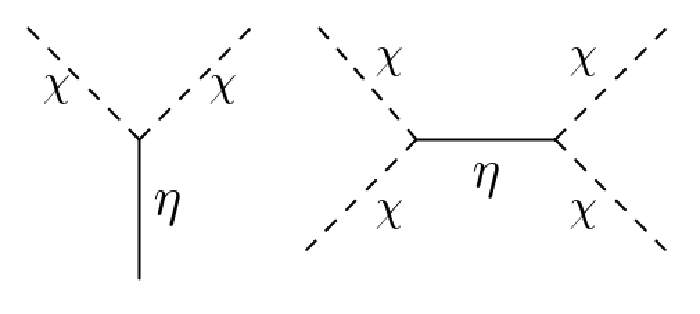
\includegraphics{Images/eqthm2.pdf}
    \caption*{}
    \label{fig:my_label}
\end{figure}
\[
M(\chi\chi\to\chi\chi)=\frac{i}{2!}4\cdot2\frac{1}{v^2}\left[\frac{(p_1\cdot p_2)(p_3\cdot p_4)}{s-m_\eta^2}+(2\xleftrightarrow[]{}3)+(2\xleftrightarrow[]{}4)\right]
\]
The scattering amplitudes are the same, so we proved the equivalence theorem.\marginnote{Su sta roba sono un po' scettico perché non mi sembra sia stato dimostrato qualcosa ma tant'è.}
\section{Self-Interacting Massive Spin-1 Particles}
These are non-abelian gauge theories and we want to generalize the U(1) case. For the abelian case, we established an equivalence between the Proca Lagrangian and gauge theories introducing the complex scalar field $\varphi(x)=ve^{i\chi(x)/v}/\sqrt{2}$ along with its non-linear constraint\\
$\varphi^\dagger(x)\varphi(x)=v^2/2$. Since it is subject to a non-linear constraint, the global U(1) symmetry cannot be linearly realized. We know there is SSB in the vacuum, where $\langle\varphi(x)\rangle=v/\sqrt{2}$ and $\chi(x)=0$, breaking U(1) to the identity.\\
\subsection{U$(N)\to$U$(N-1)$ Spontaneous Breaking}
Now we want to move to the non-abelian case, where we have $N$ complex scalar fields $\varphi_i(x)$ with the same non-linear constraint as before. We can perform a U$(N)$ transformation on these fields:
\[
\text{U}(N): \varphi(x)\to U\varphi(x)=\varphi'(x) \; U\in\text{U}(N)
\]
The new field $\varphi'(x)$ still satisfy the constraint so it is a good transformation and the U$(N)$ invariant Lagrangian is simply given by $\pazocal{L}=|\partial_\mu\varphi(x)|^2$. Again, here the symmetry is not linearly realized because of the constraint. We can write $\varphi(x)$ in the following representation:
\[
\varphi(x)=\frac{v}{\sqrt{2}}\exp{\frac{i\chi^{\hat{a}}(x)T^{\hat{a}}}{v}}\begin{pmatrix}0\\0\\\vdots\\1\end{pmatrix}
\]
where $T^{\hat{a}}$ are the \textbf{broken generators}, i.e. generators that are in U$(N)$ but not in U$(N-1)$ and they correspond to the number of NGBs. We have a total of $2N-1$ degrees of freedom, since we have $N$ fields  with 2 degrees of freedom each and one constraint: this is the number of fields we have to put in the exponential, $a=1,2,\dots,2N-1$. In the vacuum, $\chi$ is put to 0 and the field $\varphi(x)$ becomes:
\[
\varphi(x)=\frac{v}{\sqrt{2}}\begin{pmatrix}0\\0\\\vdots\\1\end{pmatrix}
\]
This vev spontaneously breaks U$(N)$ down to U$(N-1)$: how many NGBs do we have in this case? We have to count the broken generators:
\begin{align*}
& &&\text{U}(N) &&\text{U}(N-1)\\
\hline
&\#\text{generators} &&N^2 && (N-1)^2\\
&\#\text{broken generators:} &&N^2-(N-1)^2=2N-1 &&&
\end{align*}
$2N-1$ is the number of NGBs in the theory, which corresponds exactly to the number of degrees of freedom of $\chi(x)$. What happens if we promote this symmetry to local property? First we introduce $N^2$ gauge fields $A_\mu(x)$ minimally coupled to the scalar field. We expect that some of these $N^2$ gauge fields acquire mass.\marginnote{Lagrangiana schiaffata totalmente a caso e poi magia nera tra aggiunte e scatolette porca di quella troia.}
\[
\pazocal{L}=-\frac{1}{4}(F_{\mu\nu}^a)^2+|D_\mu\varphi(x)|^2
\]
U$(N-1)$ is linearly realized but what are the representations under U$(N-1)$?
\[
\begin{aligned}
&\text{U}(N)&&\text{U}(N-1)\\
&\text{Adj}&&={\color{red}\text{Adj}}+{\color{blue}\Box}+{\color{green}1}\\
&N^2&&={\color{red}(N-1)^2}+{\color{blue}2(N-1)}+{\color{green}1}
\end{aligned}
\]
How can we prove this decomposition? There are two ways:
\begin{enumerate}
    \item the adjoint representation of a unitary group can be seen as a series of $N^2$ fields times the U$(N)$ generators:
    \[
    A_\mu^A(x)T^A(x)\to\begin{pNiceArray}{cw{c}{1cm}cc}[margin]
    \Block{3-3}{\color{red}{\text{\small{$(N-1)\times(N-1)$}}}} & & & \color{blue}\vdots \\
    & & & \color{blue}\vdots \\
    & & & \color{blue}\vdots \\
    \Cdots & \Cdots & \Cdots & \tikz\draw[green,fill=green] (0,0) circle (.5ex)
    \end{pNiceArray}\quad\begin{cases}
    {\color{red}\text{Adjoint of U$(N-1)$}}\\
    {\color{blue}\text{$\Box$ of U$(N-1)$}}\\
    {\color{green}\text{Singlet of U$(N-1)$}}
    \end{cases}
    \]
    \item a field in the adjoint representation can be seen as a rank 2 tensor with indices $i,j=1,\dots,N$. If we restrict these indices to\\
    $a,b=1,\dots,N-1$ we get the adjoint.
    \[
    \begin{aligned}
    & &&\text{Adj}&&&\Box&&&&1\\
    &\phi_{ij}\to&&\phi_{ab}&&&\phi_{aN}&&&&\phi_{NN}
    \end{aligned}
    \]
\end{enumerate}
The field $\varphi(x)$ does not transform as a U$(N)$ representation because of the constraint, it does not have to have $2N$ degrees of freedom but $2N-1$: it is not $\Box$ of U$(N)$ but it contains $\Box$ of U$(N-1)$+one singlet. When we have a non-linearly realized U$(N)$ global symmetry, the complex field of this theory does not have to be a complete representation of this theory but it must contain complete multiplets of the unbroken symmetry. This is due to the fact that only linearly realized symmetries imply conserved charges which can be used to characterize the spectrum of the asymptotic states. Every asymptotic state must be a representation of the linearly realized symmetry , in this case U$(N-1)$. This $\Box+1$ we just found gives us the extra polarization we were looking for\marginnote{Ma mo' che cazzo è sta terza polarizzazione.} and together with the other 2 forms the massive vector field. We expect that the Lagrangian has $(N-1)^2$ massless gauge fields and $2N-1$ massive spin-1 particles: this is the Higgs mechanism, these $2N-1$ degrees of freedom will acquire mass. We can verify it and to do that we move to the unitary gauge, where it is possible to read the spectrum directly from the Lagrangian. To go to the unitary gauge we make a local U$(N)$ transformation on $\varphi(x)$, so that all the NGBs are put to zero.
\[
\varphi(x)\to U(\alpha(x))\varphi(x)=\frac{v}{\sqrt{2}}\begin{pmatrix}
    0\\
    \vdots\\
    0\\
    1
\end{pmatrix}
\]
The transformation $U(\alpha(x))$ is defined as $U(\alpha(x))=\exp{i\alpha^A(x)T^A}$ where $T^A$ are the generators of U$(N)$, while $T^a$ are the U$(N-1)$ unbroken generators which give us zero when acting on the column vector. Therefore, we are left only with the broken generators which correspond to what we wrote in the beginning: it is the most generic expression we can have for the field in the unitary gauge.
\[
|D_\mu\varphi(x)|^2=\left|(\partial_\mu-igA_\mu^AT^A)\frac{v}{\sqrt{2}}\begin{pmatrix}
    0\\
    \vdots\\
    0\\1
\end{pmatrix}\right|^2=\frac{g^2v^2}{2}A_\mu^{\hat{a}}A_\mu^{\hat{b}}\phi_0^TT^{\hat{a}}T^{\hat{b}}\phi_0
\]
where we denoted with $\phi_0$ the column vector and we see that only the broken generators survive. The mass matrix we will have to add is:
\[
(M^2)_{\hat{a}\hat{b}}=(gv)^2\phi_0^TT^{\hat{a}}T^{\hat{b}}\phi_0
\]
which is the Higgs mechanism for non-abelian gauge theories with broken U$(N)$ symmetry. We started our discussion with massless fields, some of them remained massless while other ones acquired mass through the Higgs mechanism. But what if we wanted a theory with all massive particles? 
\subsection{SU$(N)_L\times$SU$(N)_R\to$SU$(N)_V$ Spontaneous Breaking}
Consider $N^2$ gauge fields and $(2N-1)$ NGBs, $N^2\ge2N-1$ for $N\ge1$: hence, for $N>1$ there will always be massless particles in the theory. How do we get rid of them? We consider another example where all the NGBs are hidden and there are no massless gauge fields. Consider a theory with a global symmetry, SU$(N)_L\times$SU$(N)_R\to$SU$(N)_V$:
\[
\begin{aligned}
& &&\text{SU}(N)_L&&&\text{SU}(N)_R&&&&\text{SU}(N)_V\\
\hline
&\text{\# generators:} &&N^2-1 &&&N^2-1 &&&&N^2-1\\
&\text{\# broken generators:} &&N^2-1 &&& &&&&
\end{aligned}
\]
How can we parameterize these NGBs? We introduce the field\\
$\Sigma(x)=\exp{2i\frac{\chi^a(x)}{v}T^a}$, with $T^a$ generators of SU$(N)$ in the fundamental representation, i.e. $N\times N$ matrices. Consider now the following kinetic term:
\[
\pazocal{L}=\frac{1}{4}v^2\Tr{\partial_\mu\Sigma^\dagger\partial^\mu\Sigma}
\]
$\Sigma$ is dimensionless by definition, so it is needed to add the term $v^2$ which has dimension 2. What global symmetry do we have in this case? We can make a transformation in which $\Sigma$ is multiplied by elements of SU$(N)_L$ and SU$(N)_R$:
\[
\Sigma(x)\to L\Sigma(x)R \quad L\in\text{SU}(N)_L, R\in\text{SU}(N)_R
\]
which gives us a symmetry due to the cyclicity of the trace. In the vacuum, the fields are put to zero, so $\langle\Sigma(x)\rangle=\mathbb{1}$ breaking SU$(N)_L\times$SU$(N)_R$ to SU$(N)_V$, i.e. elements of SU$(N)_L\times$SU$(N)_R$ which preserve $\langle\Sigma(x)\rangle=\mathbb{1}$ must be equal ($L=R$), hence elements of SU$(N)_V$ by definition. But why do we work in SU$(N)$? There is an even larger symmetry given by U$(N)_L\times$U$(N)_R$ broken to U$(N)_V$. However, this results in an additional NGB and if we do the same transformation as before $\Sigma'$ will not have the same properties as $\Sigma$ because now $L$ and $R$ are not special unitary matrices anymore. We focus on SU$(N)_L\times$SU$(N)_R\to$SU$(N)_V$ because it is the symmetry realized in QCD.
\[
\text{SU}(N)_L\times\text{SU}(N)_R\times\text{U}(1)_L\times\text{U}(U)_R\to\text{SU}(N)_V\times\text{U}(1)_V
\]
The symmetry pattern of U$(1)_L\times$U$(1)_R$ can be written as U$(1)_A\times$U$(1)_V$ where the new generators are defined as:
\[
\left\{
\begin{aligned}
&T_V:=T_R+T_L\\    
&T_A:=T_R-T_L
\end{aligned}
\right.
\]
These generators are abelian, so we can always write U$(1)_L\times$U$(1)_R$=U$(1)_A\times$U$(1)_V$ but this is not true for SU$(N)$: SU$(N)_A$ does not exist because the algebra is not closed. U$(1)_V$ is just a spectator of this play because it is linearly realized, the extra NGB comes from U$(1)_A$ which is spontaneously broken.\marginnote{U$(1)_A$ is anomalous in QCD: it is a symmetry present on the classical level bur not on the quantum one.}\\
Let's get back to the case where $\Sigma(x)$ is special and unitary. We want to see the Higgs mechanism, so we make part of this symmetry local, there are two possibilities: we either make local SU$(N)_L$ or SU$(N)_R$. We decide to work with the first one, so we introduce $N^2-1$ gauge fields $A_\mu^a(x)$ and then we have to make covariant the derivative.\marginnote{If we make local SU$(N)_R$ instead the covariant derivative will have a plus sign since we are in the anti-fundamental representation.}
\[
D_\mu\Sigma=\partial_\mu\Sigma-igT^aA_\mu^A\Sigma
\]
At the end of the day, we can write the Lagrangian as:
\[
\pazocal{L}=-\frac{1}{4}(F_{\mu\nu}^a)^2+\frac{v^2}{4}\Tr{D_\mu\Sigma^\dagger D^\mu\Sigma}
\]
As usual, we move to the unitary gauge where $\Sigma(x)=\mathbb{1}$. To do that, we make a local SU$(N)$ transformation which hides all the NGBs and we obtain:
\[
\frac{v^2}{4}\Tr{D_\mu\Sigma^\dagger D^\mu\Sigma}=\frac{v^2}{4}g^2\Tr{T^aT^b}A_\mu^aA_\mu^b=\frac{1}{2}\left(\frac{vg}{2}\right)^2A_\mu^a(x)A_\mu^a(x)\Rightarrow m=\frac{gv}{2}
\]
In the last step we used the fact that $T^a$ and $T^b$ are generally normalized so that $\Tr{T^aT^b}=\delta^{ab}/2$. We observe that all the gauge fields acquire the same mass.\marginnote{If we make both SU$(N)_L$ and SU$(N)_R$ local we will have $N^2-1$ massive fields and $N^2-1$ will remain massless, but we do not want those extra massless fields.}
SU$(N)_L\times$SU$(N)_R$ is not linearly realized even if the transformation for $\Sigma$ is linear: how is that possible? We have two non-linear constraints:
\begin{enumerate}
    \item $\Sigma\Sigma^\dagger=\Sigma^\dagger\Sigma=\mathbb{1}$ results in $N^2$ constraints ($\Sigma$ is a $N\times N$ hermitian matrix)
    \item $\Tr{\log\Sigma}=0$ results in 1 constraint. This is because $\Sigma$ has to be not only unitary but also special, we are requiring that the generators are traceless.
\end{enumerate}
Finally, there will be $2N^2-N^2-1=N^2-1$ degrees of freedom which are exactly the ones we have.\\
SU$(N)_V$ is linearly realized, which means that also $\chi(x)$ transforms linearly.
\[
\Sigma\xrightarrow[]{\text{SU}(N)_V}\underbrace{e^{i\alpha^AT^A}}_{V}\underbrace{e^{2i\chi^a(x)T^a/v}}_{\Sigma}\underbrace{e^{-i\alpha^AT^A}}_{V^\dagger}=\exp{2i\chi^a(x)VT^aV^\dagger}
\]
If we write the exponential as a series we obtain exactly the transformation rule for a linearly realized symmetry. Define now:
\[
\chi^a(x)T^a\to\chi^a(x)\underbrace{VT^aV^\dagger}_{R_{ab}T^b}=\underbrace{\chi^a(x)R_{ab}}_{\chi^b(x)}T^b=\chi^b(x)T^b
\]
We proved that SU$(N)_V$ is linearly realized. However, this theory is not complete because we cannot extrapolate it at arbitrary high energies. It is a theory of $N^2-1$ self-interacting spin-1 particles, in the unitary gauge we have:
\[
\pazocal{L}=-\frac{1}{4}(F_{\mu\nu}^a)^2+\frac{1}{2}m_A^2A_\mu^aA_\mu^a
\]
\subsection{SU$(2)\times$SU$(2)\to$SU(2) Spontaneous Breaking}
Why do we switch to the formalism with $\Sigma$ when it is possible to write the Lagrangian in this way? First of all, it is not clear that it is a gauge theory while it is if we write it in terms of $\Sigma$. Moreover, $\Sigma$ contains an important information: in the scattering processes there is, at a certain energy, a probability larger than 1 as long as we are at the tree-level, we are losing perturbative unitarity. Consider the scattering of two longitudinal vectors $A_L^aA_L^b\to A_L^cA_L^d$: 
\begin{figure}[h]
    \centering
    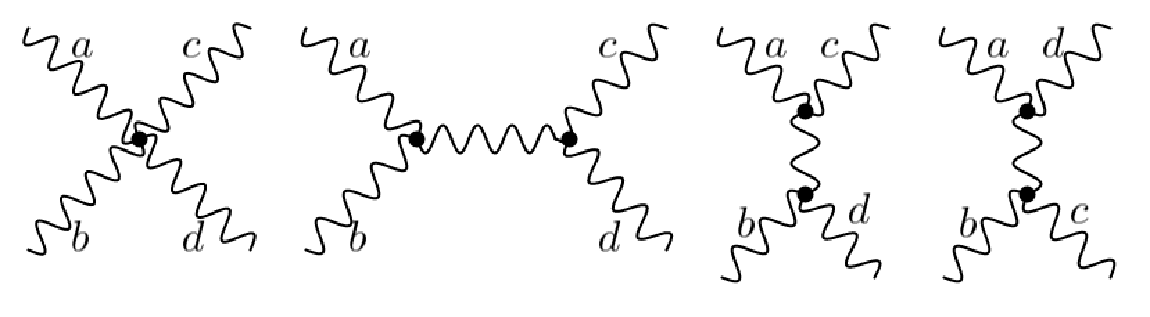
\includegraphics{Images/abcd.pdf}
    \caption{Scattering of two longitudinal vectors.}
    \label{fig:my_label}
\end{figure}if we sum all the diagrams, we find out that the total goes like $E^2$, which is obviously not good. We have to use the equivalence theorem [\refsec{eqthm}] to try to cure this growth. The theorem tells us that we can compute the scattering amplitude of this process by substituting $A_L$ with the NGB $\chi$ but to perform this calculation we have to be in the $\xi$-gauge. 
\[
\pazocal{L}=-\frac{1}{4}(F_{\mu\nu}^a)^2+\frac{v^2}{4}\Tr{D_\mu\Sigma^\dagger D^\mu\Sigma}+\text{gauge-fixing}
\]
We have to work on the trace term, let's write it explicitly:
\[
\Tr{D_\mu\Sigma^\dagger D^\mu\Sigma}=\Tr{\partial_\mu\Sigma^\dagger\partial^\mu\Sigma}+\underbrace{igA_\mu^a\Tr{-\partial_\mu\Sigma^\dagger T^a\Sigma+\Sigma^\dagger T^a\partial_\mu\Sigma}}_{=gA_\mu^a\Tr{\Sigma^\dagger T^ai\overset{\leftrightarrow}{\partial_\mu}\Sigma}=gA_\mu^AJ_\mu^a}+g^2A_\mu^aA_\mu^b\Tr{\Sigma^\dagger T^aT^b\Sigma}
\]
We want to expand this expression in powers of $\chi$, keeping only terms as high as $\chi^2$. We define $\chi:=\chi^aT^a/v$ and work in the case $N=2$ (SU$(2)\times$SU$(2)\to$SU(2)), where $T^a=\sigma^a/2$. We want to compute $igA_\mu^a\Tr{\Sigma^\dagger\frac{\sigma^a}{2}\partial_\mu\Sigma}$:
\begin{align*}
igA_\mu^a\Tr{\Sigma^\dagger\frac{\sigma^a}{2}\partial_\mu\Sigma}&\simeq igA_\mu^a\Tr{(1-i\chi-\chi^2/2+\dots)\frac{\sigma^a}{2}(i\partial_\mu\chi-\partial_\mu\chi^2/2+\dots)}\\
&=igA_\mu^A\left[\Tr{i\frac{\sigma^a}{2}\partial_\mu\chi}+\Tr{\chi\frac{\sigma^a}{2}\partial_\mu\chi-\frac{1}{2}\frac{\sigma^a}{2}\partial_\mu\chi^2}+\pazocal{O}(\chi^3)\right]
\end{align*}
Hence, it follows that:
\[
\Tr{\Sigma^\dagger\frac{\sigma^a}{2}\overset{\leftrightarrow}{\partial_\mu}\Sigma}=\frac{2i}{v}\partial_\mu\chi^a+\frac{2i}{v^2}\varepsilon^{abc}\partial_\mu\chi^b\chi^c+\pazocal{O}(\chi^3)
\]
The first term tells us that $\pazocal{L}\supset-\frac{1}{2}gv^2A_\mu^a\partial^\mu\chi^a$ which is the term we want to remove, so we choose a proper gauge-fixing term:
\[
\pazocal{L}_{GF}=-\frac{1}{2\xi}(\partial_\mu A^{\mu,a}+\frac{1}{2}\xi gv\chi^a)^2
\]
The term $\Tr{\partial_\mu\Sigma^\dagger\partial^\mu\Sigma}$ is invariant under $\Sigma\to\Sigma^\dagger$, which is equivalent to changing the sign of $\chi^a$: in the expansion of powers of $\chi$, there will only be even powers of $\chi$. To compute the kinetic term, we need to go to the 4-th order in $\chi$, so we have to expand $\Sigma$ up to the 3-rd order.
\[
\Tr{\partial_\mu\Sigma^\dagger\partial^\mu\Sigma}\simeq\Tr{(-i\partial_\mu\chi-\frac{1}{2}\partial_\mu\chi^2+\frac{i}{6}\partial_\mu\chi^3+\dots)(-i\partial_\mu\chi-\frac{1}{2}\partial_\mu\chi^2+\frac{i}{6}\partial_\mu\chi^3+\dots)}
\]
The term $\chi^2$ is equal to $\chi^2=\frac{\chi^a\sigma^a}{2}\frac{\chi^bsigma^b}{2}=\frac{\chi^a\chi^b}{v^2}\frac{1}{2}\{\sigma^a\sigma^b\}$ so we can write:
\[
\frac{v^2}{4}\Tr{\partial_\mu\Sigma^\dagger\partial^\mu\Sigma}=\frac{1}{2}(\partial_\mu\chi^a)^2+\frac{1}{6v^2}[(\chi^a\partial_\mu\chi^a)^2-\chi^a\chi^a(\partial_\mu\chi^b\partial^\mu\chi^b)+\dots]
\]
The last term above is the only one contributing to the scattering at this order of energy, with a contribution$\simeq E^2/v^2$. The full Lagrangian with the gauge-fixing term is now the following:
\begin{align*}
\pazocal{L}+\pazocal{L}_{GF}&=-\frac{1}{4}(F_{\mu\nu}^a)^2-\frac{1}{2\xi}(\partial_\mu A^{\mu,a})^2+\frac{m_A^2}{2}A_\mu^aA_\mu^a+\frac{1}{2}(\partial_\mu\chi^a)^2-\frac{1}{2}m_A^2\xi(\chi^a)^2\\
&-\frac{1}{2}g\varepsilon^{abc}A_\mu^a\partial_\mu\chi^b\chi^c+\frac{1}{6v^2}\left[(\chi^a\partial_\muchi^a)^2-\chi^a\chi^b(\partial_\mu\chi^b\partial^\mu\chi^b)\right]+\pazocal{O}[\chi^b,A\chi^3] \quad m_a=\frac{gv}{2}
\end{align*}
Now that we have the Lagrangian, it is possible to compute the amplitude but of a special case: $\chi^a\chi^b\to\chi^a\chi^b$.\marginnote{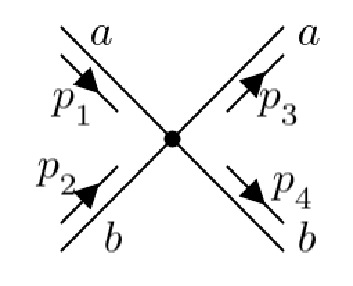
\includegraphics{Images/abab.pdf}\\
Diagram at the first order in perturbation theory.}
\[
M(\chi^a\chi^b\to\chi^a\chi^b)=\frac{2i}{6v^2}[-(p_1-p_3)_\mu(p_2-p_4)^\mu-2\cdot2p_2\cdot p_4]
\]
We have to look at the kinematic of this process and it tells us that:
\[
\left\{
\begin{aligned}
&p_1+p_2=p_3+p_4\\
&p_1-p_3=-(p_2-p_4)
\end{aligned}
\right.
\to
\left\{
\begin{aligned}
&(p_1-p_3)^2=t\\
&(p_2-p_4)^2=t=2m_A^2-2p_2\cdot p_4
\end{aligned}
\right.
\]
Hence, the amplitude becomes:
\begin{equation}
\labeq{chi}
M(\chi^a\chi^b\to\chi^a\chi^b)=\frac{i}{3v^2}[t+2(t-2m_A^2)]+\dots=\frac{it}{v^2}+\dots\sim\frac{E^2}{v^2}:=g^2(E)
\end{equation}
It is possible to interpret this amplitude as the coupling squared, which grows with the energy. The strength of this interaction increases as the energy increases, therefore there will be a certain value of energy for which perturbative theory does not hold anymore: is it possible to estimate this value? We consider the 1-loop contribution \marginnote{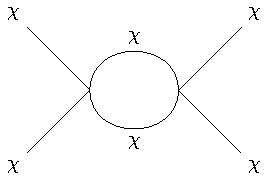
\includegraphics[]{Images/chiloop.pdf}\\
1-loop diagram.} which gives a contribution $\sim\frac{E^2}{v^2}\frac{E^2}{16\pi^2v^2}$, so the perturbative expansion will be something like:
\[
g^2(E)+g^2(E)\frac{g^2(E)}{16\pi^2}+\dots
\]
This perturbative series breaks when $\frac{g^2(E)}{16\pi^2}\sim\pazocal{O}(1)$, which corresponds to $E_{max}\approx4\pi v$: at this energy we lose perturbative unitarity. 
\section{Higgs Boson}
What do we do with this theory when it breaks at high energies? There are two possibilities:
\begin{enumerate}
    \item modify the theory, so that it becomes mathematically complete. To do that, we need to add more degrees of freedom
    \item keep it as an effective field theory, valid upon a certain energy
\end{enumerate}
We start with the first option, adding degrees of freedom. It is possible to add just one to make the theory complete, the \textbf{Higgs boson}. It is exactly what we have done for the U(1) case:
\[
\varphi(x)=\frac{v}{\sqrt{2}}\exp{i\chi(x)/v} \quad \varphi^\dagger(x)\varphi(x)=\frac{v^2}{2}
\]
$\varphi(x)$ was not a complete representation of U(1), it has to be a complex scalar representation with 2 degrees of freedom, hence the non-linear constraint. We have also seen that it is possible to incorporate one extra degree of freedom to make the theory linearly realized:
\[
\varphi(x)=\frac{v+h(x)}{\sqrt{2}}\exp{i\chi(x)/v}
\]
In this way we can realize a real U(1) linear transformation. However, this theory is not renormalizable because the coupling goes like $E^{-2}$.\marginnote{From power counting, we know that theories with couplings which go like a negative power of the energy are not renormalizable.} Moreover, we have a global symmetry not linearly realized. These two observations are correlated: if we can add a degree of freedom to make the theory renormalizable we can prove that the theory can be extrapolated at arbitrary high energies. \\
Let's see how to realize a complete representation. On the field $\Sigma$ we had the following conditions:
\[
\underbrace{\Sigma^\dagger\Sigma=\Sigma\Sigma^\dagger=\mathbb{1}}_{\text{4 conditions}} \quad \underbrace{\det\Sigma=1}_{\text{1 condition}}
\]
A $2\times2$ complex matrix has 8 degrees of freedom: 8-5=3 Adj of SU$(2)_V$. What is the smallest possible dimension of a SU$(2)_L\times$SU$(2)_R$ representation? Let $\Phi$ a generic $2\times2$ matrix which transforms as $\Phi\to L\Phi R^\dagger$: this has 8 degrees of freedom, 5 more than the ones we had before. We need to impose some linear constraint on $\Phi$. We use the fact that SU(2) has pseudo-real representations, i.e. real up to a unitary transformation. Let $\Psi$ be $\Box$ of SU(2), pseudo real: if $\Psi^*$ transforms as a doublet of SU(2), then it is a real representation. However, $\Psi$ is pseudo-real so we add a unitary transformation:
\[
U\Psi^*=i\sigma^2\Psi^*:=\Psi^c
\]
In the SU(2) case, the unitary transformation is $i\sigma^2$, therefore we have:
\[
\left\{
\begin{aligned}
&\Psi\to\exp{i\alpha^a\sigma^a}\Psi\\
&\Psi^c\to\exp{i\alpha^a\sigma^a}\Psi^c
\end{aligned}
\right.
\]
Suppose now that $\Phi$ transforms as $\Phi\to L\Phi R^\dagger$, $\Phi^c=i\sigma^2\Phi^*(-i\sigma^2)$ will transform as $\Phi^c\to L\Phi^c R^\dagger$: it transforms in the same way as $\Phi$. We can impose $\Phi=\Phi^c$, throwing away 4 degrees of freedom since it gives us 4 conditions. Now $\mathcal{H}:=\Phi$\marginnote{The change of notation in the last few lines:\\

\includegraphics[]{Images/parkour.jpg}\\
Parkour!} and it is possible to define $\mathcal{H}\to L\mathcal{H}R^\dagger$, $\mathcal{H}=i\sigma^2\mathcal{H}^*(-i\sigma^2)$ this is the reality condition from which it follows that $\mathcal{H}=\varphi(x)\Sigma(x)$. $\mathcal{H}$ has 4 degrees of freedom, 3 in $\Sigma(x)$ and 1 in $\varphi(x)$. In general $\mathcal{H}$ is a $2\times2$ matrix which can always be written as $\mathcal{H}=a_0\mathbb{1}+ia_i\sigma^i$, but the reality condition implies that $a_0$ and $a_i$ must be real.
\begin{align*}
&\mathcal{H}^\dagger\mathcal{H}=(a_0\mathbb{1}-ia_i\sigma^i)(a_0\mathbb{1}+ia_i\sigma^i)=a_0^2\mathbb{1}+a_ia_j\sigma^i\sigma^j\\
&=a_0^2\mathbb{1}+\frac{a_ia_j}{2}\{\sigma^i,\sigma^j\}=(a_0^2+a_i^2)\mathbb{1}
\end{align*}
$\mathcal{H}^\dagger\mathcal{H}$ is the identity, we could have seen it directly from the definition $\mathcal{H}=\varphi(x)\Sigma(x)$. At this point we have to write the Lagrangian for $\mathcal{H}$ and obtain the Feynman rules, i.e. the interactions.
\[
\pazocal{L}=-\frac{1}{4}(F_{\mu\nu}^a)^2+\frac{1}{4}\Tr{(D_\mu\mathcal{H})^\dagger(D^\mu\mathcal{H})}
\]
SU$(2)_L\times$SU$(2)_R$ has to be spontaneously broken, so we must add a potential $V(\mathcal{H})$ to the Lagrangian.\marginnote{We add it with a minus sign so that we can recover the usual Mexican hat. Andale! Andale!}
\[
V(\mathcal{H})=-\frac{\mu^2}{4}\Tr{\mathcal{H}^\dagger\mathcal{H}}+\frac{\lambda}{16}(\Tr{\mathcal{H}^\dagger\mathcal{H}})^2=-\frac{\mu^2}{2}\varphi^2(x)+\frac{\lambda}{4}\varphi^4(x)
\]
It follows that $\langle\varphi(x)\rangle=v=\sqrt{\mu^2/\lambda}$, so we can write $\varphi(x)=v+h(x)$ where $h(x)$ is the Higgs boson (fluctuations around the vev). Now we have to substitute the expression for $\mathcal{H}$ in the $\xi$-gauge and find the interactions. From the trace term we obtain the kinetic term for the Higgs boson, while from the potential the mass term for $h(x)$ and its interactions.
\begin{align*}
&\bullet D_\mu\mathcal{H}=\partial_\mu\varphi\Sigma+\varphi D_\mu\Sigma\\
&\bullet \Tr{(D_\mu\mathcal{H})^\dagger(D^\mu\mathcal{H})}=2(\partial_\mu\varphi)^2\Tr{\Sigma\Sigma^\dagger}+\varphi^2\Tr{D_\mu\Sigma^\dagger D^\mu\Sigma}
\end{align*}
From the last trace, the main interaction we find for the Higgs boson is $\frac{1}{2}(\partial_\mu\chi^2)^2\frac{h}{4}$, which gives a contribution to the scattering amplitude. This contribution is what cures $g^2(E)$.\\
It is possible to write the full Lagrangian as:
\[
\pazocal{L}=-\frac{1}{4}(F_{\mu\nu}^a)^2+\frac{1}{2}(\partial_\mu\varphi)^2+\frac{\mu^2}{2}\varphi^2-\frac{\lambda}{4}\varphi^4+\frac{1}{4}\varphi^2\Tr{(D_\mu\Sigma)^\dagger(D^\mu\Sigma)}
\]
Let's look at the potential: if we look for the minima, we find\\
$\langle\varphi\rangle=v=\sqrt{\mu^2/\lambda}$. This means that SU$(2)_L\times$SU$(2)_R$ is a broken symmetry, broken to SU$(2)_V$. It is now possible to define the field $\varphi(x)$ as the vev+a certain excitation $h(x)$ with $m_h^2=2\mu^2$. This is the 4-th degree of freedom for the massive radial excitation, the other 3 are in $\Sigma$ and parameterize the excitation around the valley of minima.
\begin{align*}
\pazocal{L}&=-\frac{1}{4}(F_{\mu\nu}^a)^2+\frac{1}{2}(\partial_\mu h(x))^2+\frac{1}{2}m_h^2h^2(x)-\lambda vh^3(x)-\frac{\lambda}{4}h^4(x)\\
&+\frac{v^2}{4}\left(1+\frac{h(x)}{v}\right)^2\Tr{(D_\mu\Sigma)^\dagger(D^\mu\Sigma)}+\text{constant terms}
\end{align*}
We have $h(x)$ as a self-interacting massive field and it interacts through the last term with the NGB $\chi^a$ contained in $\Sigma$. We want to understand this interaction and see how this fixes the dependency $E^2$ of the scattering amplitude of $\chi^a\chi^b\to\chi^a\chi^b$. This gives us the diagram depicted on the side \marginnote[-3cm]{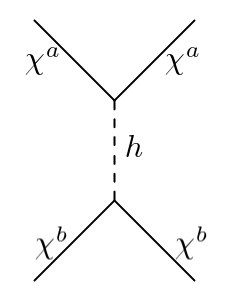
\includegraphics{Images/aahbb.png}}:
\begin{align*}
M_h(\chi^a\chi^b\to\chi^a\chi^b)&=\frac{i^2}{2!v^2}2\cdot2\cdot2(p_1\cdot p_3)(p_2\cdot p_4)\frac{i}{(p_1-p_3)^2-m_h^2}\\
&=\frac{-i}{t-m_h^2}(t-2m_A)^2\frac{1}{v^2}=-\frac{it}{v^2}+\dots
\end{align*}
This contribution is exactly the same as the one from $\chi$ [\refeq{chi}] with opposite sign, hence they cancel each other and the scattering amplitude is constant at high energies. \raisebox{-\mydepth}{{
\includegraphics[height=1.1\baselineskip]{Images/smile.jpg}}}

If we have a spontaneously broken symmetry G$\to$H, the fields must form a complete multiplet of H, not of G. There are two possibilities to spontaneously break G to H:
\begin{itemize}
    \item fields form complete multiplets of G but at the minimum of the potential G$\to$H.\marginnote{The symmetry G is recovered at high energies, $E\gg v$} What we have is then a massive spin-1 particles theory which at high energies can be interpreted as massless spin-1 particles+scalar. This means that at high energies the spin-1 massive theory has to be interpreted as a gauge theory where the fields are representations of G.
    \item fields do not form a complete representation of G but only of H: they cannot be extrapolated at high energies, the massive spin-1 particles theory collapses at some point because there is one less degree of freedom, there is no $h(x)$. It is an effective theory, there is a cut-off $\Lambda\approx4\pi v$.
\end{itemize}

\end{document}


%QFT beyond tree-level (QED a 1 -loop con Barducci)
%Symmetries and conservation laws (spontaneous symmetry breaking and Higgs mechanism)
%Quick intro to non-abelian gauge theories
%Effective field theories
%Intro to the SM